% Options for packages loaded elsewhere
\PassOptionsToPackage{unicode}{hyperref}
\PassOptionsToPackage{hyphens}{url}
%
\documentclass[
]{book}
\usepackage{amsmath,amssymb}
\usepackage{lmodern}
\usepackage{iftex}
\ifPDFTeX
  \usepackage[T1]{fontenc}
  \usepackage[utf8]{inputenc}
  \usepackage{textcomp} % provide euro and other symbols
\else % if luatex or xetex
  \usepackage{unicode-math}
  \defaultfontfeatures{Scale=MatchLowercase}
  \defaultfontfeatures[\rmfamily]{Ligatures=TeX,Scale=1}
  \setmainfont[]{Libre Baskerville}
\fi
% Use upquote if available, for straight quotes in verbatim environments
\IfFileExists{upquote.sty}{\usepackage{upquote}}{}
\IfFileExists{microtype.sty}{% use microtype if available
  \usepackage[]{microtype}
  \UseMicrotypeSet[protrusion]{basicmath} % disable protrusion for tt fonts
}{}
\makeatletter
\@ifundefined{KOMAClassName}{% if non-KOMA class
  \IfFileExists{parskip.sty}{%
    \usepackage{parskip}
  }{% else
    \setlength{\parindent}{0pt}
    \setlength{\parskip}{6pt plus 2pt minus 1pt}}
}{% if KOMA class
  \KOMAoptions{parskip=half}}
\makeatother
\usepackage{xcolor}
\usepackage[left=4cm, right=3cm, top=2.5cm, bottom=2.5cm]{geometry}
\usepackage{listings}
\newcommand{\passthrough}[1]{#1}
\lstset{defaultdialect=[5.3]Lua}
\lstset{defaultdialect=[x86masm]Assembler}
\usepackage{longtable,booktabs,array}
\usepackage{calc} % for calculating minipage widths
% Correct order of tables after \paragraph or \subparagraph
\usepackage{etoolbox}
\makeatletter
\patchcmd\longtable{\par}{\if@noskipsec\mbox{}\fi\par}{}{}
\makeatother
% Allow footnotes in longtable head/foot
\IfFileExists{footnotehyper.sty}{\usepackage{footnotehyper}}{\usepackage{footnote}}
\makesavenoteenv{longtable}
\usepackage{graphicx}
\makeatletter
\def\maxwidth{\ifdim\Gin@nat@width>\linewidth\linewidth\else\Gin@nat@width\fi}
\def\maxheight{\ifdim\Gin@nat@height>\textheight\textheight\else\Gin@nat@height\fi}
\makeatother
% Scale images if necessary, so that they will not overflow the page
% margins by default, and it is still possible to overwrite the defaults
% using explicit options in \includegraphics[width, height, ...]{}
\setkeys{Gin}{width=\maxwidth,height=\maxheight,keepaspectratio}
% Set default figure placement to htbp
\makeatletter
\def\fps@figure{htbp}
\makeatother
\setlength{\emergencystretch}{3em} % prevent overfull lines
\providecommand{\tightlist}{%
  \setlength{\itemsep}{0pt}\setlength{\parskip}{0pt}}
\setcounter{secnumdepth}{5}
\newlength{\cslhangindent}
\setlength{\cslhangindent}{1.5em}
\newlength{\csllabelwidth}
\setlength{\csllabelwidth}{3em}
\newlength{\cslentryspacingunit} % times entry-spacing
\setlength{\cslentryspacingunit}{\parskip}
\newenvironment{CSLReferences}[2] % #1 hanging-ident, #2 entry spacing
 {% don't indent paragraphs
  \setlength{\parindent}{0pt}
  % turn on hanging indent if param 1 is 1
  \ifodd #1
  \let\oldpar\par
  \def\par{\hangindent=\cslhangindent\oldpar}
  \fi
  % set entry spacing
  \setlength{\parskip}{#2\cslentryspacingunit}
 }%
 {}
\usepackage{calc}
\newcommand{\CSLBlock}[1]{#1\hfill\break}
\newcommand{\CSLLeftMargin}[1]{\parbox[t]{\csllabelwidth}{#1}}
\newcommand{\CSLRightInline}[1]{\parbox[t]{\linewidth - \csllabelwidth}{#1}\break}
\newcommand{\CSLIndent}[1]{\hspace{\cslhangindent}#1}
\usepackage{float}
\floatplacement{figure}{H}
\usepackage{booktabs}
\usepackage{setspace}
\usepackage{fontspec}
\onehalfspacing
\usepackage{xcolor}
\usepackage{titlesec}
\usepackage{xfrac}
% Make caption labels bold: https://bookdown.org/yihui/rmarkdown-cookbook/latex-extra.html
\usepackage[labelfont={bf}]{caption} 
% force floats forward: https://bookdown.org/yihui/rmarkdown-cookbook/figure-placement.html
\usepackage{flafter}
% https://tex.stackexchange.com/questions/279/how-do-i-ensure-that-figures-appear-in-the-section-theyre-associated-with
\usepackage{placeins}
\lstset{
  breaklines=true
}
\usepackage{wrapfig}
\usepackage{lipsum}
\usepackage{caption}
\captionsetup[figure]{font=small}
% following code copied from https://bookdown.org/yihui/rmarkdown-cookbook/figure-placement.html#fnref10 
\renewcommand{\topfraction}{.85}
\renewcommand{\bottomfraction}{.7}
\renewcommand{\textfraction}{.15}
\renewcommand{\floatpagefraction}{.66}
\setcounter{topnumber}{3}
\setcounter{bottomnumber}{3}
\setcounter{totalnumber}{4}

%% https://stackoverflow.com/questions/3275770/modifying-section-to-make-it-colorful-with-latex
%\usepackage{color}
%\titleformat{\section}
%{\color{red}}


% https://tex.stackexchange.com/questions/10320/section-and-subsection-colors-using-titlesec
%\makeatletter
%\newcommand*\@secondofsix[6]{#2}
%\newcommand{\addtotitleformat}{%
%  \@ifstar{\addtotitleformat@star}{\addtotitleformat@nostar}}
%\newcommand\addtotitleformat@nostar[2]{%
%  \PackageError{titlesec}{non starred form of \string\addtotitleformat\space not supported}{}}
%\newcommand\addtotitleformat@star[2]{%
%  \expandafter\expandafter\expandafter\expandafter
%  \expandafter\expandafter\expandafter\def
%  \expandafter\expandafter\expandafter\expandafter
%  \expandafter\expandafter\expandafter\@currentsection@font
%  \expandafter\expandafter\expandafter\expandafter
%  \expandafter\expandafter\expandafter{%
%    \expandafter\expandafter\expandafter\@secondofsix
%       \csname ttlf@\expandafter\@gobble\string#1\endcsname}%
%  \titleformat*{#1}{\@currentsection@font#2}%
%}
%\makeatother
%
%\addtotitleformat*{\section}{\Huge\color{red}}
%\addtotitleformat*{\subsection}{\sffamily\color{blue}}
\usepackage{titling}
\usepackage{subcaption}
\pretitle{\begin{center} 
\includegraphics[width=2in,height=2in]{/Users/brettell/Documents/Repositories/PhD-thesis/book/figs/title/Arms_PembrokeCollege_Cambridge.pdf}\LARGE\\ \bigskip \bigskip \bigskip }
\posttitle{\end{center}}
\predate{\begin{center}}
\postdate{\end{center} \centering \begin{figure}[!tpb] \centering \begin{subfigure}{0.49 \linewidth} \centering \vfill \includegraphics[height=0.45in]{/Users/brettell/Documents/Repositories/PhD-thesis/book/figs/title/cambridge_university2.pdf} \end{subfigure} \hfill \begin{subfigure}{0.49 \linewidth} \centering \includegraphics[height=0.55in]{/Users/brettell/Documents/Repositories/PhD-thesis/book/figs/title/EMBL_EBI_Logo_black.pdf} \end{subfigure} \end{figure} }
\usepackage{float}
\usepackage{booktabs}
\usepackage{longtable}
\usepackage{array}
\usepackage{multirow}
\usepackage{wrapfig}
\usepackage{colortbl}
\usepackage{pdflscape}
\usepackage{tabu}
\usepackage{threeparttable}
\usepackage{threeparttablex}
\usepackage[normalem]{ulem}
\usepackage{makecell}
\usepackage{xcolor}
\ifLuaTeX
  \usepackage{selnolig}  % disable illegal ligatures
\fi
\IfFileExists{bookmark.sty}{\usepackage{bookmark}}{\usepackage{hyperref}}
\IfFileExists{xurl.sty}{\usepackage{xurl}}{} % add URL line breaks if available
\urlstyle{same} % disable monospaced font for URLs
\hypersetup{
  pdftitle={Japanese courage: a genetic analysis of complex traits in medaka fish and humans},
  pdfauthor={Ian Narain Brettell},
  hidelinks,
  pdfcreator={LaTeX via pandoc}}

\title{Japanese courage: a genetic analysis of complex traits in medaka fish and humans}
\author{Ian Narain Brettell}
\date{15 September 2022}

\begin{document}
\maketitle

{
\setcounter{tocdepth}{1}
\tableofcontents
}
\hypertarget{about}{%
\chapter*{About}\label{about}}
\addcontentsline{toc}{chapter}{About}

\textbf{Japanese courage: a genetic analysis of complex traits in medaka fish and humans}

This thesis primarily explores how an individual's genes interact with the genes of their social companions to create differences in behaviour, using the Japanese medaka fish as a model organism. Chapter 1 sets out the introduction to the diverse topics covered in this thesis.

Chapter 2 describes several genomic characteristics of the Medaka Inbred Kiyosu-Karlsruhe (MIKK) panel, which comprises 80 inbred lines of medaka that were bred from a wild population residing in Kiyosu, southern Japan. In this chapter I plot the inbreeding trajectory of the MIKK panel, and analyse its evolutionary relationship with other previously established inbred medaka strains; degree of homozygosity; rate of linkage disequilibrium decay; repeat content; and structural variation, all which relate to its utility for the genetic mapping of complex traits.

In Chapter 3, I use a custom behavioural assay to characterise and classify bold-shy behaviours in 5 previously established inbred medaka lines. Here I describe the assay, assess its robustness against confounding factors, and apply a hidden markov model (HMM) to classify the fishes' behaviours across a spectrum of boldness-shyness based on their distance and angle of travel between time points. I describe how the different lines differ in their behaviours over the course of the assay (a direct genetic effect) and how the behaviour of a single ``reference'' line (\emph{iCab}) differs in the presence of different lines (a social genetic effect).

In Chapter 4, I explain how I applied this behavioural assay to the MIKK panel in order to identify lines that diverge in both their own bold-shy behaviours (the direct genetic effect) and the extent to which they transmit those behaviours onto their tank partners (the social genetic effect). I then describe how we used those divergent lines as the parental lines in a multi-way F2 cross in an attempt to isolate the genetic variants that are associated with both direct and social genetic effects.

In Chapter 5 I describe the bioinformatic processes and genetic association models used to map the variants associated with differences in the period of somite development, based on a separate F2 cross between the southern Japanese \emph{iCab} strain, and the northern Japanese \emph{Kaga} strain.

Finally, in Chapter 6, I compare and rank all complex traits in the GWAS Catalog based on the extent to which their associated alleles vary across global human populations, using the Fixation Index (Fst) as a metric and the 1000 Genomes dataset as a sample of global genetic variation. In this chapter I set out the bioinformatic pipelines used to process the data, present the distributions of Fst for trait-associated alleles across the genome, and use the Kolmogorov-Smirnov test to compare the distributions of Fst across different traits.

Altogether, this thesis describes some of the genomic characteristics of both medaka fish and humans, and how those variations relate to differences in complex traits, with a particular focus on the genetic causes of adaptive behaviours and the transmission of those behaviours onto one's social companions.

\hypertarget{acknowledgements}{%
\chapter*{Acknowledgements}\label{acknowledgements}}
\addcontentsline{toc}{chapter}{Acknowledgements}

Thanks.

\hypertarget{preface}{%
\chapter*{Preface}\label{preface}}
\addcontentsline{toc}{chapter}{Preface}

\hypertarget{abstract}{%
\chapter*{Abstract}\label{abstract}}
\addcontentsline{toc}{chapter}{Abstract}

\hypertarget{MIKK-F2-chap}{%
\chapter{Genetic linkage study of bold/shy behaviours in the MIKK panel}\label{MIKK-F2-chap}}

\chaptermark{MIKK panel behaviour}

The purpose of the study described in this chapter was to run the behavioural analysis described in Chapter \ref{Pilot-chap} over the MIKK panel described in Chapter \ref{MIKK-genomes-chap}, identify the lines that diverged in both (a) their own behaviour; and (b) the level of transmission of their behaviour onto their \emph{\definecolor{iCab_424B4D}{HTML}{424B4D}\textcolor{iCab_424B4D}{iCab}} reference tank partner, and then use them as the parental strains in an F2 cross to attempt to identify the specific genetic loci associated with those differences.

\hypertarget{data-collection---f0-generation}{%
\section{Data collection - F0 generation}\label{data-collection---f0-generation}}

In November 2019 I traveled to the fish facility managed by our collaborators, the Loosli Group at KIT in Karlsruhe, Germany, and over the course of 11 days from 11 to 21 November 2019, I ran the behavioural assay described in Chapter \ref{pilot-data-collection} another 206 times. I again used the \emph{\definecolor{iCab_424B4D}{HTML}{424B4D}\textcolor{iCab_424B4D}{iCab}} strain as the reference fish, and for the test fish I used either an individual from one of the MIKK panel lines, individuals captured from the same Kiyosu population as the MIKK panel but permitted to breed freely within a separate tank in the facility (`Kiyosu closed-capture', or `\textbf{Kiyosu CC}'), or individuals from a related but different species of medaka from the Philippines, \emph{Oryzias luzonensis}. I ensured that I performed at least 2 assay runs of 4 individuals each on two different days for each MIKK panel line that was available, generating a minimum of 8 test fish replicates per line. As there were four pairs of fish in the test tank during each run, the complete dataset comprises 824 videos of pairs of fish, which I further divided by assay component (open field and novel object) to create 1648 videos.

I again used the software \emph{idtrackerai} (Romero-Ferrero et al. 2019) to track the movement of the fishes across frames of each video. After adjusting the software parameters for each video to maximise the number of frames that were successfully tracked, I was left with 1610 out of the 1648 videos (\textasciitilde97.7\%) where both fishes were tracked over at least 85\% of frames, and I only included these 1610 videos in the downstream analysis. The first question to address was whether the MIKK panel lines differed in their behaviours. I therefore computed each individual fish's mean speed (measured as the distance traveled in pixels per 0.08 seconds) over the course of the full 20-minute video, grouped them by line, and plotted the results presented in \textbf{Figure \ref{fig:mikk-mean-speed}}. I continue to use the same order and colour palette for the MIKK panel lines as in this Figure throughout the rest of this Chapter.



\begin{figure}
\includegraphics[width=1\linewidth]{figs/mikk_behaviour/line_mean_speed_0.08_all} \caption{Mean speed of the MIKK panel and other strains over the course of the entire 20-minute video (measured as the distance traveled in pixels per 0.08 seconds). \emph{\definecolor{iCab_424B4D}{HTML}{424B4D}\textcolor{iCab_424B4D}{iCab}} fishes in the \emph{\definecolor{iCab_424B4D}{HTML}{424B4D}\textcolor{iCab_424B4D}{iCab}}-\emph{\definecolor{iCab_424B4D}{HTML}{424B4D}\textcolor{iCab_424B4D}{iCab}} control condition are at the top, the MIKK panel lines are sorted by their group median, and the Kiyosu closed capture and \emph{O. luzonensis} fishes are at the bottom.}\label{fig:mikk-mean-speed}
\end{figure}

This figure shows that there are clear differences between some MIKK panel lines at the extremes, and that the lines differ in the amount of within-line variance observed (shown plotted against the lines' median speed in \textbf{Figure \ref{fig:mikk-mean-speed-variance}}). These figures acted as a general guide to determine which lines to select as the parental strains in the F2 cross. To identify genetic variants directly associated with bold-shy behaviours, I sought to select lines that showed either high or low levels of movement, and preferably low within-line variance.



\begin{figure}
\includegraphics[width=1\linewidth]{figs/mikk_behaviour/line_mean_speed_variance_0.08_all} \caption{Line median (vertical axis) and line variance (horizontal axis) for individual mean speed (pixels per 0.08 seconds) across the full 20-minute video (i.e.~both the open field and novel object assay components).}\label{fig:mikk-mean-speed-variance}
\end{figure}

To illustrate the differences between certain lines in terms of both direct and social genetic effects, in \textbf{Figure \ref{fig:extreme-paths}} I have plotted the tracked paths for 3 lines 5 minutes into the 10-minute open field assay component: the slowest line \definecolor{22-1 (‘David’)_FB737A}{HTML}{FB737A}\textcolor{22-1 (‘David’)_FB737A}{22-1 (‘David’)},\footnote{In almost all cases, David remained as still (and captivating) as Michelangelo's statue for the entirety of the assay.} one of the other slowest lines \definecolor{18-2 (‘Elsa’)_FF66A6}{HTML}{FF66A6}\textcolor{18-2 (‘Elsa’)_FF66A6}{18-2 (‘Elsa’)},\footnote{Similar to David, Elsa was also Frozen, but far more charismatic.} and the fastest line . The fishes are coloured by their line, with \emph{\definecolor{iCab_424B4D}{HTML}{424B4D}\textcolor{iCab_424B4D}{iCab}} in dark grey. There appears to be a social genetic effect when comparing the behaviour of \emph{\definecolor{iCab_424B4D}{HTML}{424B4D}\textcolor{iCab_424B4D}{iCab}} when paired with the similarly slow-moving lines and \definecolor{18-2 (‘Elsa’)_FF66A6}{HTML}{FF66A6}\textcolor{18-2 (‘Elsa’)_FF66A6}{18-2 (‘Elsa’)}. At the other extreme, line \definecolor{10-1 (‘Janeway’)_F8766D}{HTML}{F8766D}\textcolor{10-1 (‘Janeway’)_F8766D}{10-1 (‘Janeway’)}\footnote{Janeway appeared to spend most of its time moving at warp speed.} has moved extremely quickly, spending much of its time moving along the boundaries of their test tanks. I understand from our collaborator Felix Loosli, a fish behaviour expert, that this movement along the boundaries of a tank is typical of medaka when introduced to a novel environment, and we observe it too with \emph{\definecolor{iCab_424B4D}{HTML}{424B4D}\textcolor{iCab_424B4D}{iCab}} when it is paired with line \definecolor{22-1 (‘David’)_FB737A}{HTML}{FB737A}\textcolor{22-1 (‘David’)_FB737A}{22-1 (‘David’)}.



\begin{figure}
\includegraphics[width=1\linewidth]{figs/mikk_behaviour/path_plot_22-1_18-2_10-1_300} \caption{Path plots for lines 22-1 (\textbf{A}), 18-2 (\textbf{B}) and 10-1 (\textbf{C}) 5 minutes into the open field assay for the first (left) and second (right) run with each line. The paths of \emph{\definecolor{iCab_424B4D}{HTML}{424B4D}\textcolor{iCab_424B4D}{iCab}} individuals are coloured in dark grey, with the other lines depicted in their representative colours.}\label{fig:extreme-paths}
\end{figure}

Although lines \definecolor{22-1 (‘David’)_FB737A}{HTML}{FB737A}\textcolor{22-1 (‘David’)_FB737A}{22-1 (‘David’)} and \definecolor{10-1 (‘Janeway’)_F8766D}{HTML}{F8766D}\textcolor{10-1 (‘Janeway’)_F8766D}{10-1 (‘Janeway’)} were the most extreme in terms of mean speed, I ruled them out of selection for the F2 cross for the following reasons. Our collaborators informed us that through a separate analysis on heartbeat phenotypes across the MIKK panel, they discovered that the heart of line \definecolor{22-1 (‘David’)_FB737A}{HTML}{FB737A}\textcolor{22-1 (‘David’)_FB737A}{22-1 (‘David’)} often stops beating for up to minutes at a time. This may explain the lack of movement observed during our assay. The behaviours they exhibit may therefore not represent a phenotype related to the boldness-shyness axis, but rather an extreme phenotype of a particular organ system. Our collaborators are, however, using this line in a separate F2 cross investigating heart phenotypes.

On the other hand, line \definecolor{10-1 (‘Janeway’)_F8766D}{HTML}{F8766D}\textcolor{10-1 (‘Janeway’)_F8766D}{10-1 (‘Janeway’)} appeared to habituate to the open field assay component by slowing down, rather than speeding up (\textbf{Figure \ref{fig:10-1-dens}}). That is to say, as the assay progressed, they slowed down their movement, and this suggests that their typical response to stress is to move faster rather than slower. However, as I am using speed as a proxy for boldness (where a quicker habituation to the assay, indicated by an increase in movement, suggests greater boldness), this would create difficulties in attributing a functional interpretation of behaviours in the F2 individuals, and for this reason I excluded line \definecolor{10-1 (‘Janeway’)_F8766D}{HTML}{F8766D}\textcolor{10-1 (‘Janeway’)_F8766D}{10-1 (‘Janeway’)}.



\begin{figure}
\includegraphics[width=1\linewidth]{figs/mikk_behaviour/select_0.08_15_10-1_dge} \caption{Tile and density plots for line \definecolor{10-1 (‘Janeway’)_F8766D}{HTML}{F8766D}\textcolor{10-1 (‘Janeway’)_F8766D}{10-1 (‘Janeway’)}, showing the reduction in the frequency of higher-movement states over the course of the open field assay component (\textbf{A} and \textbf{B}), with the novel object assay component (\textbf{C} and \textbf{D}) for comparison.}\label{fig:10-1-dens}
\end{figure}

\clearpage

\hypertarget{hmm-states}{%
\section{HMM states}\label{hmm-states}}

To explore the behaviours of the MIKK panel at a finer resolution, as for the pilot study described in Chapter \ref{Pilot-chap}, I again applied a Hidden Markov Model (\textbf{HMM}) to classify the fishes' movements based on their distance and angle of travel between time intervals. I used the same method to select the best choice of time interval and number of states (\textbf{Figure \ref{fig:mikk-param-comp}}).



\begin{figure}
\includegraphics[width=1\linewidth]{figs/mikk_behaviour/compare_params} \caption{Comparison between HMM parameters. Horizontal axis: Mean concordance between states assigned by HMMs through a 2-fold cross-validation process. Vertical axis: Kruskal-Wallis statistic comparing strains based on the proportion of time spent in each HMM state, summed across all states. Size of points correspond to the interval, in seconds, between which the distance and angle of travel was calculated (Methods).}\label{fig:mikk-param-comp}
\end{figure}

Here I observed the same phenomenon where the parameter combinations that performed the best showed an asymmetry between some states that would make interpretation difficult. For example, a time interval of 0.08 seconds combined with a state space of 17 caused state 4 to appear to get carved out of state 3 (\textbf{Figure \ref{fig:mikk-hmm-asym}}).



\begin{figure}
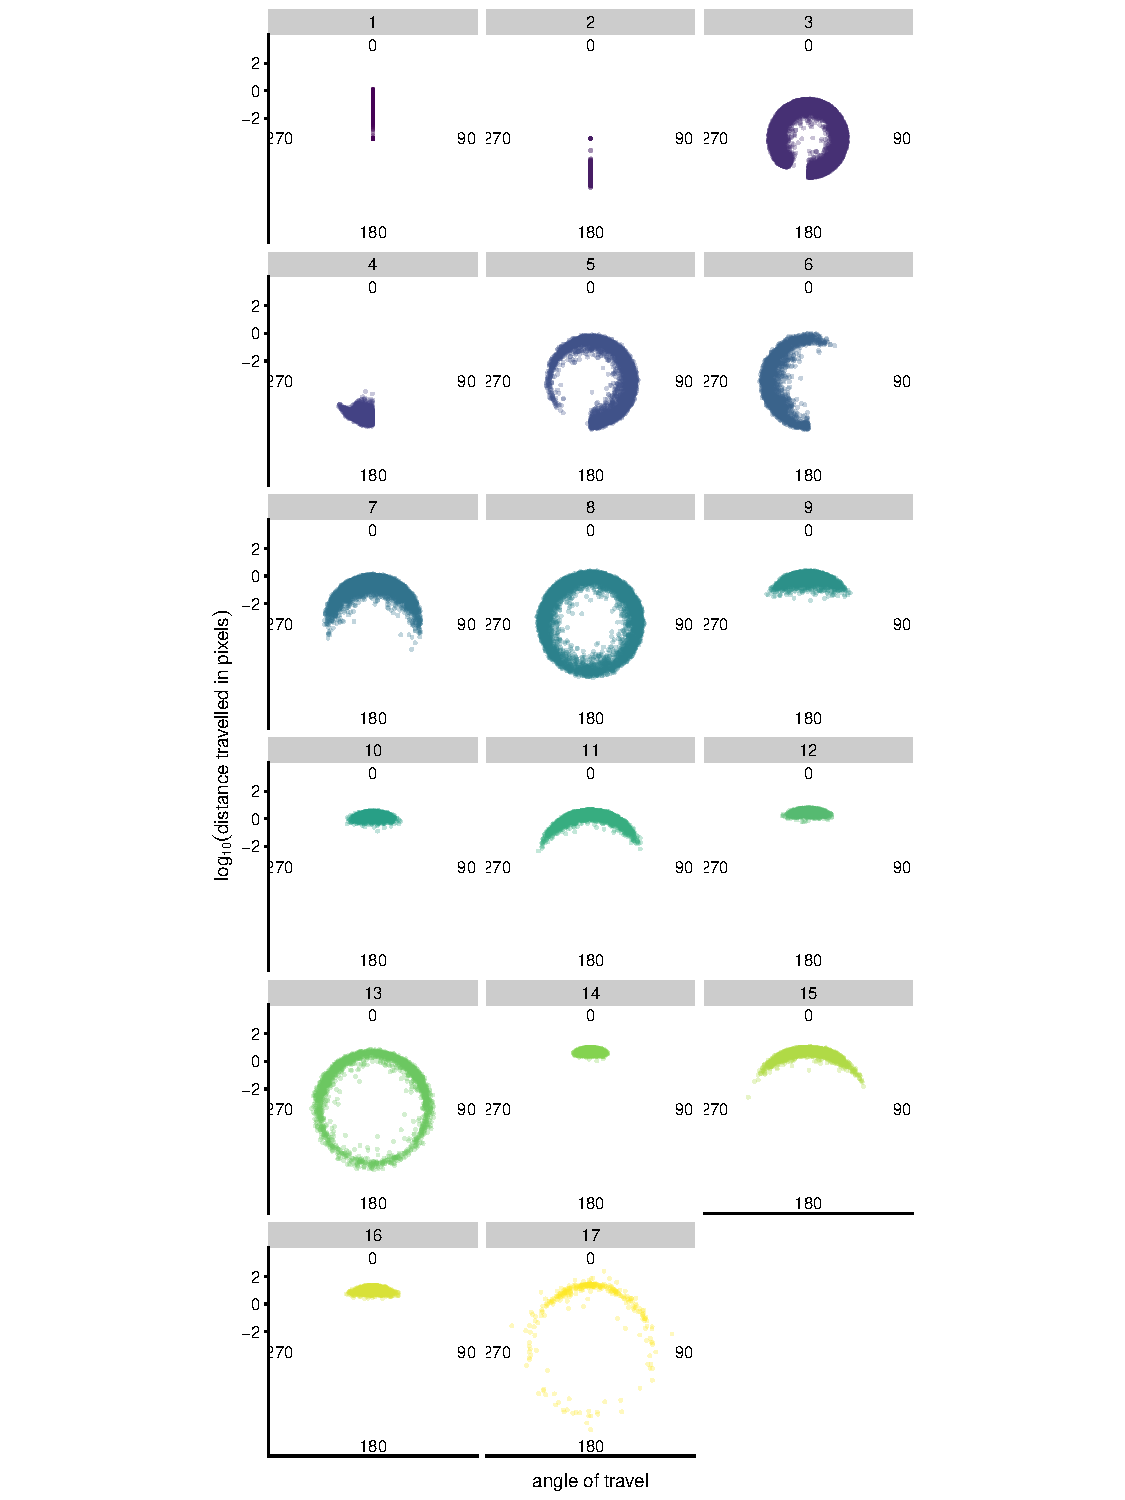
\includegraphics[width=1\linewidth]{figs/mikk_behaviour/0.08_17_polar_all_dge} \caption{Based on the concordance analysis results set out in Figure \ref{fig:mikk-param-comp} above, the best apparent combination of parameters -- 0.08 time interval with a 17-state space -- created an asymmetry between states 3 and 4, which would cause difficulties in interpreting their biological relevance.}\label{fig:mikk-hmm-asym}
\end{figure}

The best combination of parameters \emph{without} this asymmetry was a time interval of 0.05 seconds with a state space of 15 (see the polar plots for the states in \textbf{Appendix \ref{fig:hmm-states-05}}). However, due to a glitch in the video recording software, several videos recorded on 13 November 2019 were incorrectly recorded with a frame rate of 14 instead of the desired 30. The insufficient number of frames for those videos meant that it was impossible to measure the distance and angle of travel between a time interval as low as 0.05 seconds. So that these videos could be included in the dataset, I accordingly selected the combination of 15 states and a 0.08-second interval for all downstream analyses (\textbf{Figure \ref{fig:mikk-hmm-sym}}).



\begin{figure}
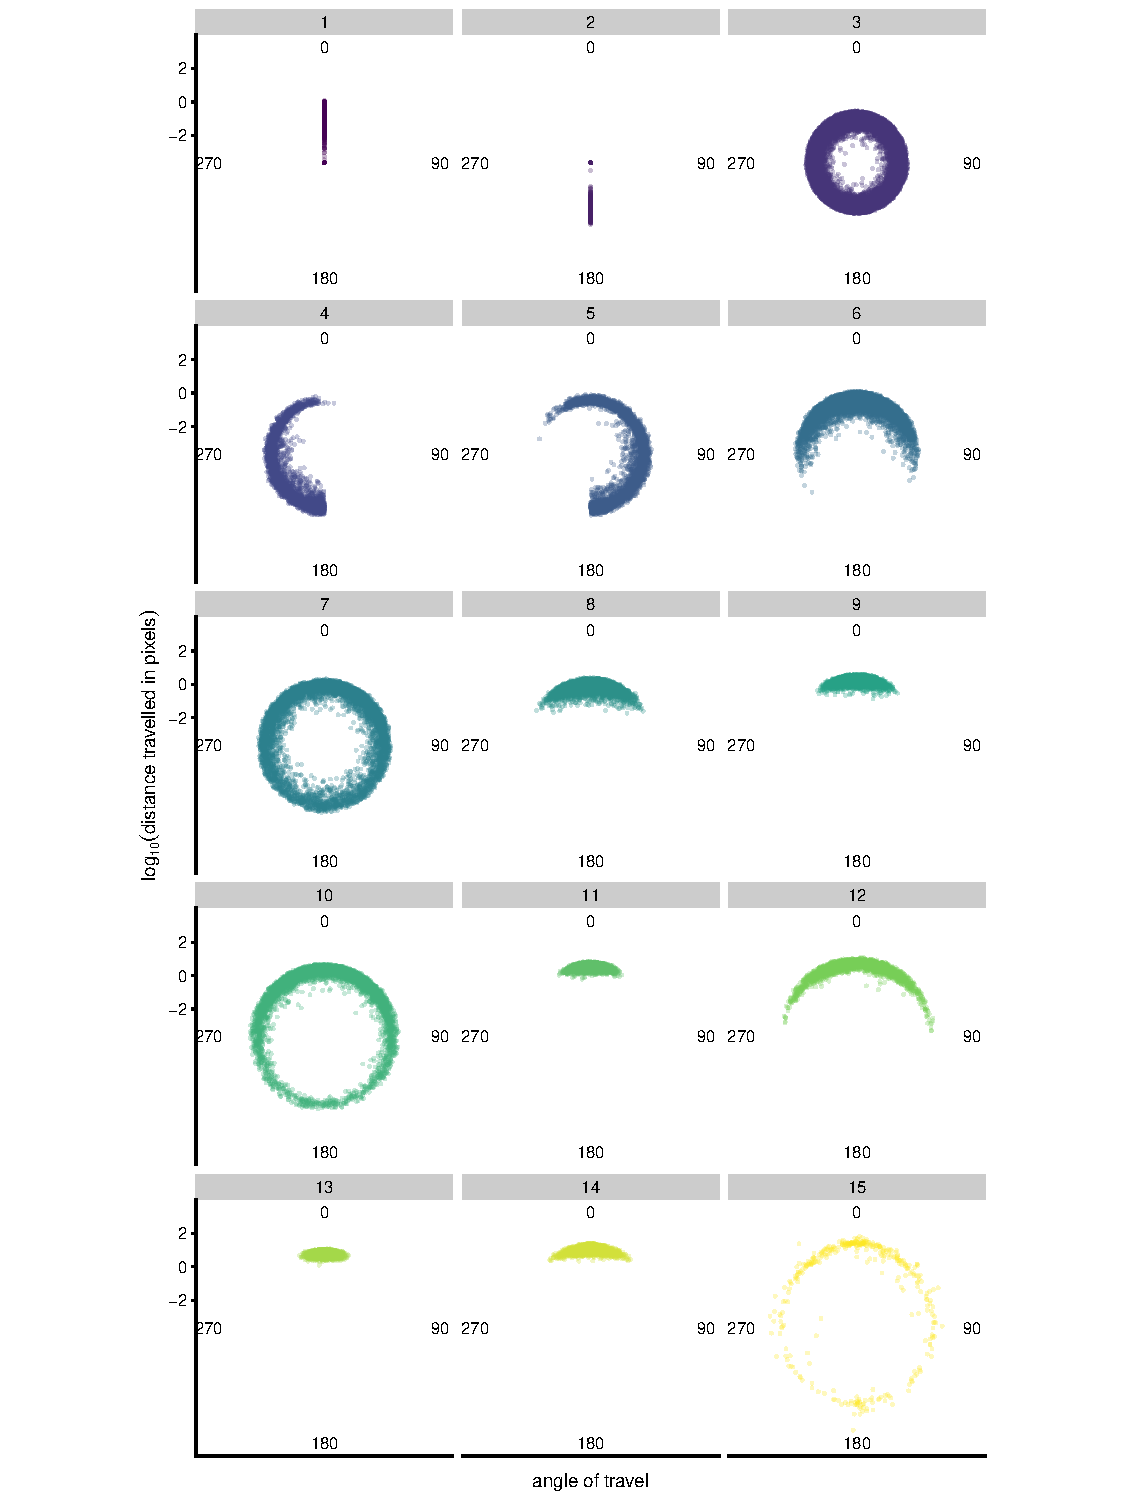
\includegraphics[width=1\linewidth]{figs/mikk_behaviour/0.08_15_polar_all_dge} \caption{The HMM states used for the downstream analysis, with the model classified based on the distance of travel (log\textsubscript{10} pixels, radial axis) and angle of travel (angle). A straight forward movement would sit around 0°, a left movement around 270°, and a right movement around 90°.}\label{fig:mikk-hmm-sym}
\end{figure}

\clearpage

\hypertarget{social-genetic-effects}{%
\section{Social genetic effects}\label{social-genetic-effects}}

As discussed above, in this project our traits of interest include not only direct genetic behaviours, but also social genetic behaviours. I therefore sought to identify the MIKK panel lines that transmit their behaviour onto the reference \emph{\definecolor{iCab_424B4D}{HTML}{424B4D}\textcolor{iCab_424B4D}{iCab}} tank partners either to the greatest or least extent. I refer to this transmission of behaviour as ``\textbf{\emph{charisma}}'', to capture the element of behavioural influence. I formulated two methods to measure charisma, which I refer to as a) HMM state co-occupancy; and b) reference deviation. The first, HMM state co-occupancy, measures the proportions of time that the \emph{\definecolor{iCab_424B4D}{HTML}{424B4D}\textcolor{iCab_424B4D}{iCab}} reference fish spends in the same HMM state as its tank partner. The second, deviation of the reference fishes' behaviour from the behaviour exhibited in the control condition, seeks to quantify the extent to which the \emph{\definecolor{iCab_424B4D}{HTML}{424B4D}\textcolor{iCab_424B4D}{iCab}}'s behaviour changes when partnered with each MIKK panel line.

\hypertarget{state-co-occupancy}{%
\subsection{State co-occupancy}\label{state-co-occupancy}}

\textbf{Figure \ref{fig:F0-sge-cooc-box}} sets out the proportions of total time for each assay sub-component that each pair of individual fish spent in the same HMM state, grouped by line and ranked in the same order as their group median for individual mean speed as shown above in \textbf{Figure \ref{fig:mikk-mean-speed}}. \textbf{\ref{fig:F0-sge-cooc-box}A} shows the data as boxplots, with \(p\)-values from the Kruskal-Wallis test comparing all groups. \textbf{Figure \ref{fig:F0-sge-cooc-box}B} shows the same data but with each group's median represented by columns to make it easier to compare group medians. Of the slower-moving lines, \definecolor{8-2 (‘Gail’)_FF699C}{HTML}{FF699C}\textcolor{8-2 (‘Gail’)_FF699C}{8-2 (‘Gail’)}\footnote{Named after Gail the Snail, the slow but curiously captivating character from \emph{It's Always Sunny in Philadelphia}.} and \definecolor{18-2 (‘Elsa’)_FF66A6}{HTML}{FF66A6}\textcolor{18-2 (‘Elsa’)_FF66A6}{18-2 (‘Elsa’)} tend to show relatively higher state co-occupancy in the open field component, but during the novel object component, the slow-moving line \definecolor{139-4_FF61CC}{HTML}{FF61CC}\textcolor{139-4_FF61CC}{139-4} has the highest median co-occupancy of all lines. Of the faster-moving lines, \definecolor{43-2_F17D50}{HTML}{F17D50}\textcolor{43-2_F17D50}{43-2} and \definecolor{13-2_F57A5F}{HTML}{F57A5F}\textcolor{13-2_F57A5F}{13-2} showed the highest state co-occupancy during the open field assay component. However, the moderate-to-fast line \definecolor{21-2 (‘Amelia’)_49B500}{HTML}{49B500}\textcolor{21-2 (‘Amelia’)_49B500}{21-2 (‘Amelia’)}\footnote{Named after the fast and charismatic Amelia Earhart.} had relatively high state co-occupancy during both assay components.



\begin{figure}
\includegraphics[width=1\linewidth]{figs/mikk_behaviour/0.08_15_cooc_box_all} \caption{Frequency of HMM state co-occupancy}\label{fig:F0-sge-cooc-box}
\end{figure}

To visualise which states are driving the higher co-occupancy measures, for a selection of lines I generated a heatmap of the states occupied simultaneously by the \emph{\definecolor{iCab_424B4D}{HTML}{424B4D}\textcolor{iCab_424B4D}{iCab}} reference and MIKK test fishes, combining the observations for all individuals within each test fish group (\textbf{Figure \ref{fig:F0-sge-cooc-heat}}). When \emph{\definecolor{iCab_424B4D}{HTML}{424B4D}\textcolor{iCab_424B4D}{iCab}} is paired with \definecolor{18-2 (‘Elsa’)_FF66A6}{HTML}{FF66A6}\textcolor{18-2 (‘Elsa’)_FF66A6}{18-2 (‘Elsa’)} or \definecolor{8-2 (‘Gail’)_FF699C}{HTML}{FF699C}\textcolor{8-2 (‘Gail’)_FF699C}{8-2 (‘Gail’)}, the fishes most frequently occupy states 3 or 1 in both open field and novel object components. In pairings with line \definecolor{139-4_FF61CC}{HTML}{FF61CC}\textcolor{139-4_FF61CC}{139-4}, while the test fishes remain in the still states 1 or 3 during the open field assay, \emph{\definecolor{iCab_424B4D}{HTML}{424B4D}\textcolor{iCab_424B4D}{iCab}} tends to be moving much faster in states 11 and 13. However, during the novel object component, they co-occupy state 3 more than in any other combination. This general pattern is observed with line \definecolor{14-2_F066EA}{HTML}{F066EA}\textcolor{14-2_F066EA}{14-2} as well, albeit to a lesser extent. For \definecolor{38-2 (‘Mark’)_00C08B}{HTML}{00C08B}\textcolor{38-2 (‘Mark’)_00C08B}{38-2 (‘Mark’)},\footnote{Line 38-2 appears to have intermediate measures for both movement and charisma, causing us to affectionately refer to it as the ``boring'' line, and then later to christen it after Mark Corrigan from \emph{Peep Show}.} the fishes tend not to show a strong preference for co-occupying a particular state for either assay component, but the diagonal spread indicates that they tend to move at similar speeds. When paired with the faster moving \definecolor{21-2 (‘Amelia’)_49B500}{HTML}{49B500}\textcolor{21-2 (‘Amelia’)_49B500}{21-2 (‘Amelia’)}, the novel object component appears to accentuate the co-occupancy of state 3 that is also observed in the open field component. Finally, when paired with line \definecolor{40-1 (‘Max’)_93AA00}{HTML}{93AA00}\textcolor{40-1 (‘Max’)_93AA00}{40-1 (‘Max’)},\footnote{Line 40-1 and its sibling line 40-2 both appeared to be preternaturally bold, like the siblings Max and Moritz from Wilhelm Busch's eponymous story (Busch 2015).} in both assay components, both fishes show a strong preference for the faster-moving states.



\begin{figure}
\includegraphics[width=1\linewidth]{figs/mikk_behaviour/0.08_15_cooc_heatmap} \caption{Heatmaps for a selection of MIKK panel lines (including those ultimately selected as the parental strains in the F2 cross) showing the frequency of HMM states simultaneously occupied by the reference (x-axis) and test (y-axis) fishes during the open field (\textbf{A}) and novel object (\textbf{B}) assay components, aggregated over all replicates for each line.}\label{fig:F0-sge-cooc-heat}
\end{figure}

\hypertarget{deviation-of-from-its-control-condition}{%
\subsection{\texorpdfstring{Deviation of \emph{\definecolor{iCab_424B4D}{HTML}{424B4D}\textcolor{iCab_424B4D}{iCab}} from its control condition}{Deviation of  from its control condition}}\label{deviation-of-from-its-control-condition}}

The second method for quantifying the level of behavioural transmission from test fish to \emph{\definecolor{iCab_424B4D}{HTML}{424B4D}\textcolor{iCab_424B4D}{iCab}} reference fish was to determine the proportion of time that the \emph{\definecolor{iCab_424B4D}{HTML}{424B4D}\textcolor{iCab_424B4D}{iCab}} spent in a particular state when paired with another \emph{\definecolor{iCab_424B4D}{HTML}{424B4D}\textcolor{iCab_424B4D}{iCab}}, and then quantify the degree to which those proportions change when in the presence of a fish from another line (\textbf{Figure \ref{fig:F0-sge-deviation}}). \textbf{Figure \ref{fig:F0-sge-deviation}A} presents boxplots for state frequencies for all \emph{\definecolor{iCab_424B4D}{HTML}{424B4D}\textcolor{iCab_424B4D}{iCab}} individuals in \emph{\definecolor{iCab_424B4D}{HTML}{424B4D}\textcolor{iCab_424B4D}{iCab}}-\emph{\definecolor{iCab_424B4D}{HTML}{424B4D}\textcolor{iCab_424B4D}{iCab}} pairings. I further calculated the state frequencies for all \emph{\definecolor{iCab_424B4D}{HTML}{424B4D}\textcolor{iCab_424B4D}{iCab}} reference fishes for all other MIKK line pairings. For each combination of assay component, line-pairing, and HMM state, I then ran Welch's t-test (Ruxton 2006) comparing the proportions of time the \emph{\definecolor{iCab_424B4D}{HTML}{424B4D}\textcolor{iCab_424B4D}{iCab}} individuals spent in that state when paired with another \emph{\definecolor{iCab_424B4D}{HTML}{424B4D}\textcolor{iCab_424B4D}{iCab}}, against the proportions of time the \emph{\definecolor{iCab_424B4D}{HTML}{424B4D}\textcolor{iCab_424B4D}{iCab}} reference individuals spent in that state when paired with a different MIKK line. I then summed the t-statistics across states to generate a single metric for each combination of line and assay component, and plotted the results in \textbf{Figure \ref{fig:F0-sge-deviation}B}.



\begin{figure}
\includegraphics[width=1\linewidth]{figs/mikk_behaviour/0.08_15_deviation} \caption{Deviation of state frequency for \emph{\definecolor{iCab_424B4D}{HTML}{424B4D}\textcolor{iCab_424B4D}{iCab}} reference fishes when paired with MIKK panel lines relative to when paired with another \emph{\definecolor{iCab_424B4D}{HTML}{424B4D}\textcolor{iCab_424B4D}{iCab}}. \textbf{A}: Boxplots of HMM state frequency for \emph{\definecolor{iCab_424B4D}{HTML}{424B4D}\textcolor{iCab_424B4D}{iCab}} individuals when paired with another \emph{\definecolor{iCab_424B4D}{HTML}{424B4D}\textcolor{iCab_424B4D}{iCab}}. \textbf{B}: Summed absolute t-statistics (Welch's t-test) comparing the proportions of time \emph{\definecolor{iCab_424B4D}{HTML}{424B4D}\textcolor{iCab_424B4D}{iCab}} spent in each state when paired with another \emph{\definecolor{iCab_424B4D}{HTML}{424B4D}\textcolor{iCab_424B4D}{iCab}}, against when paired with a MIKK panel line.}\label{fig:F0-sge-deviation}
\end{figure}

The first thing to note in this Figure is that \emph{\definecolor{iCab_424B4D}{HTML}{424B4D}\textcolor{iCab_424B4D}{iCab}}'s deviations from its behaviour exhibited in the control condition tend to be smaller when paired with faster-moving fishes. This was expected given \emph{\definecolor{iCab_424B4D}{HTML}{424B4D}\textcolor{iCab_424B4D}{iCab}} is also a faster-moving fish, but it strengthens the observation that when paired with slower-moving fishes, those tank partners are causing the \emph{\definecolor{iCab_424B4D}{HTML}{424B4D}\textcolor{iCab_424B4D}{iCab}} reference fish to move slower than they would otherwise. Of the slower-moving MIKK lines, \definecolor{4-2_FC61D4}{HTML}{FC61D4}\textcolor{4-2_FC61D4}{4-2} and \definecolor{14-2_F066EA}{HTML}{F066EA}\textcolor{14-2_F066EA}{14-2} causing the largest deviations of the \emph{\definecolor{iCab_424B4D}{HTML}{424B4D}\textcolor{iCab_424B4D}{iCab}} reference fishes' behaviours from their control condition behaviour in the open field and novel object components respectively. I also observe large deviations for the moderately-moving \definecolor{106-2_00B9E3}{HTML}{00B9E3}\textcolor{106-2_00B9E3}{106-2} and \definecolor{71-1_00BECD}{HTML}{00BECD}\textcolor{71-1_00BECD}{71-1} during the novel object components. There are no clear outliers for either assay component for any of the faster moving lines.

\hypertarget{selection-of-lines-for-the-f2-cross}{%
\section{Selection of lines for the F2 cross}\label{selection-of-lines-for-the-f2-cross}}

On the basis of the above findings, I selected 6 MIKK panel lines as the parental lines for the F2 cross (\textbf{Figure \ref{fig:F0-line-mean-speed-var-select}}). Conceptually, I sought to select lines that diverged on two measures: a) bold-shy behaviours; and b) the extent to which the lines transmitted their behaviours onto their tank partners.

As \emph{\definecolor{iCab_424B4D}{HTML}{424B4D}\textcolor{iCab_424B4D}{iCab}} is a fast-moving line, it was more difficult to detect instances where fast-moving MIKK panel lines were influencing its behaviour. I was therefore more confident of identifying slow-movement/high-charisma lines, and so to increase the likelihood of identifying genetic variants that are responsible for a stronger transmission of slow-moving behaviours, I chose two slow-movement/high-charisma lines for the F2 cross: \definecolor{18-2 (‘Elsa’)_FF66A6}{HTML}{FF66A6}\textcolor{18-2 (‘Elsa’)_FF66A6}{18-2 (‘Elsa’)} and \definecolor{8-2 (‘Gail’)_FF699C}{HTML}{FF699C}\textcolor{8-2 (‘Gail’)_FF699C}{8-2 (‘Gail’)}. In the event that both lines possessed the same genetic variants that influence this behavioural transmission trait, it would vastly increase the power of detecting it during the genetic linkage analysis. Both these lines were one of the most slow-moving lines, had high levels of state co-occupancy during both assay components, and \definecolor{18-2 (‘Elsa’)_FF66A6}{HTML}{FF66A6}\textcolor{18-2 (‘Elsa’)_FF66A6}{18-2 (‘Elsa’)} caused a high level of deviation from the \emph{\definecolor{iCab_424B4D}{HTML}{424B4D}\textcolor{iCab_424B4D}{iCab}} control condition.



\begin{figure}
\includegraphics[width=1\linewidth]{figs/mikk_behaviour/line_mean_speed_variance_selected} \caption{Line median (vertical axis) and line variance (horizontal axis) for individual mean speed across the full 20-minute video (i.e.~both the open field and novel object assay components) as shown above in Figure \ref{fig:mikk-mean-speed-variance}, now coloured only for the lines selected as the parental strains for the F2 cross.}\label{fig:F0-line-mean-speed-var-select}
\end{figure}

For the slow-movement/low-charisma line, I selected \definecolor{50-2 (‘Patrick’)_BB81FF}{HTML}{BB81FF}\textcolor{50-2 (‘Patrick’)_BB81FF}{50-2 (‘Patrick’)} which exhibited a moderately slow level of movement, low within-line variance for mean speed, and low measures for both state co-occupancy and \emph{\definecolor{iCab_424B4D}{HTML}{424B4D}\textcolor{iCab_424B4D}{iCab}} deviation. For the high-movement/high-charisma line, I selected \definecolor{21-2 (‘Amelia’)_49B500}{HTML}{49B500}\textcolor{21-2 (‘Amelia’)_49B500}{21-2 (‘Amelia’)}. Despite its high within line variance (\textbf{Figure \ref{fig:F2-time-dge-of}}), this potentially made it easier to detect its social genetic effects, as the slower-moving individuals appeared to transmit those behaviours strongly to their \emph{\definecolor{iCab_424B4D}{HTML}{424B4D}\textcolor{iCab_424B4D}{iCab}} tank partners, giving it a high score among fast-moving lines for state co-occupancy across both assay components. For the high-movement/low-charisma line I selected \definecolor{40-1 (‘Max’)_93AA00}{HTML}{93AA00}\textcolor{40-1 (‘Max’)_93AA00}{40-1 (‘Max’)}, as it has low within-line variance, and low-to-moderate metrics for state co-occupancy and \emph{\definecolor{iCab_424B4D}{HTML}{424B4D}\textcolor{iCab_424B4D}{iCab}} deviation. However, I note that these measures may be confounded by the possibility that \definecolor{40-1 (‘Max’)_93AA00}{HTML}{93AA00}\textcolor{40-1 (‘Max’)_93AA00}{40-1 (‘Max’)} behaves in a similar way to \emph{\definecolor{iCab_424B4D}{HTML}{424B4D}\textcolor{iCab_424B4D}{iCab}}, which would be difficult to determine whether it was behaving differently.

In addition to these extreme lines, I also selected a line that was intermediate for both traits in an attempt to avoid breeding incompatibilities that might arise from attempting to cross lines with such divergent behavioural traits. For this purpose I selected line \definecolor{38-2 (‘Mark’)_00C08B}{HTML}{00C08B}\textcolor{38-2 (‘Mark’)_00C08B}{38-2 (‘Mark’)} for its intermediate speed, low within-line variance for mean speed, and intermediate measures for HMM state co-occupancy and \emph{\definecolor{iCab_424B4D}{HTML}{424B4D}\textcolor{iCab_424B4D}{iCab}} deviation.

The selection of parental lines for the F2 cross indicating their putative position across the two axes of interest (movement, and behavioural transmission or `charisma') are set out below in \textbf{Figure \ref{fig:F0-line-select-schema}}.



{[}FOR EASE OF REFERRING TO THE LINES I GIVE THEM NAMES -- DO THAT AT THE START{]}

\begin{figure}
\includegraphics[width=1\linewidth]{figs/mikk_behaviour/line_selection_schema} \caption{Schema of the MIKK panel lines selected as the parental strains for the multi-way F2 cross, indicating their intended position across the two axes of interest (movement, and behavioural transmission or `charisma').}\label{fig:F0-line-select-schema}
\end{figure}

\clearpage

\hypertarget{direct-genetic-effects}{%
\section{Direct genetic effects}\label{direct-genetic-effects}}

With these lines selected, I ran a similar analysis to what I described in \ref{Pilot-chap}, where I ran multi-way ANOVAs to determine whether certain lines differed in the proportions of time they spent in these HMM states, while including the date of assay, time of assay, tank quadrant and tank side as covariates. \textbf{Table \ref{tab:mikk-dge-F0}} sets out the states which showed a significant difference between these 6 lines, with p-values adjusted for the False Discovery Rate (\textbf{FDR}).

\begin{table}

\caption{\label{tab:mikk-dge-F0}Significant differences in the proportion of time spent in each HMM state across test fish lines selected for the F2 cross for the open field and novel object assay components.}
\centering
\begin{tabular}[t]{llll}
\toprule
Assay & State & Variance explained (\%) & p-value (FDR-adjusted)\\
\midrule
\cellcolor{gray!6}{open field} & \cellcolor{gray!6}{3} & \cellcolor{gray!6}{21.53} & \cellcolor{gray!6}{2.67e-03}\\
open field & 4 & 23.28 & 1.60e-02\\
\cellcolor{gray!6}{open field} & \cellcolor{gray!6}{5} & \cellcolor{gray!6}{20.61} & \cellcolor{gray!6}{3.15e-02}\\
open field & 10 & 29.06 & 1.41e-03\\
\cellcolor{gray!6}{open field} & \cellcolor{gray!6}{12} & \cellcolor{gray!6}{24.91} & \cellcolor{gray!6}{1.45e-02}\\
\addlinespace
open field & 14 & 29.52 & 1.29e-03\\
\cellcolor{gray!6}{novel object} & \cellcolor{gray!6}{1} & \cellcolor{gray!6}{16.21} & \cellcolor{gray!6}{1.90e-02}\\
novel object & 2 & 15.14 & 4.86e-02\\
\cellcolor{gray!6}{novel object} & \cellcolor{gray!6}{4} & \cellcolor{gray!6}{26.90} & \cellcolor{gray!6}{5.21e-03}\\
novel object & 5 & 27.84 & 4.27e-03\\
\addlinespace
\cellcolor{gray!6}{novel object} & \cellcolor{gray!6}{10} & \cellcolor{gray!6}{23.73} & \cellcolor{gray!6}{2.81e-02}\\
\bottomrule
\end{tabular}
\end{table}

\textbf{Figures \ref{fig:F2-time-dge-of}} and \textbf{\ref{fig:F2-time-dge-no}} highlight the states that showed significant differences in the proportions of time that these lines spent in those states for the open field and novel object assay components respectively. In both figures, \textbf{A} highlights the significant states, \textbf{B} shows how the individuals moved through those states over the course of the 10-minute assay component, and \textbf{C} shows the densities of the significant states within each line. For the open field component, although the tile plots show a notable level of variance within each line, the density plots clarify how the three slow-moving lines (\definecolor{8-2 (‘Gail’)_FF699C}{HTML}{FF699C}\textcolor{8-2 (‘Gail’)_FF699C}{8-2 (‘Gail’)}, \definecolor{18-2 (‘Elsa’)_FF66A6}{HTML}{FF66A6}\textcolor{18-2 (‘Elsa’)_FF66A6}{18-2 (‘Elsa’)} and \definecolor{50-2 (‘Patrick’)_BB81FF}{HTML}{BB81FF}\textcolor{50-2 (‘Patrick’)_BB81FF}{50-2 (‘Patrick’)}) spent little time in the fast-moving states 10, 12 and 14 relative to the fast-moving lines. Interestingly, the intermediate line \definecolor{38-2 (‘Mark’)_00C08B}{HTML}{00C08B}\textcolor{38-2 (‘Mark’)_00C08B}{38-2 (‘Mark’)} tended to transition into these states around the middle of the video, presumably a period of habituating to the new environment.



\begin{figure}
\includegraphics[width=1\linewidth]{figs/mikk_behaviour/select_0.08_15_dge_of} \caption{Differences between MIKK F0 lines in the HMM states they occupied during the \emph{open field} assay component. \textbf{A}: 15 HMM states with panels coloured red to indicate significant differences between MIKK F0 lines in the proportion of time spent in those states. \textbf{B}: Transitions between HMM states across time for each individual test fish, grouped by MIKK line Tiles are coloured by the state most frequently occupied by each fish within 2-second intervals. \textbf{C}: Densities within each MIKK line for the occupation of states that significantly differed between strains (colour), with other states consolidated (grey).}\label{fig:F2-time-dge-of}
\end{figure}

During the novel object component the HMM states that showed significant differences between lines were mostly restricted to the slow-moving states with the exception of state 10, which most clearly distinguishes the slow-moving lines from the intermediate- and fast-moving lines. Again, the intermediate line \definecolor{38-2 (‘Mark’)_00C08B}{HTML}{00C08B}\textcolor{38-2 (‘Mark’)_00C08B}{38-2 (‘Mark’)} shows a sharp drop in the occupation of the slow moving states after a period of habituation.



\begin{figure}
\includegraphics[width=1\linewidth]{figs/mikk_behaviour/select_0.08_15_dge_no} \caption{Differences between MIKK F0 lines in the HMM states they occupied during the \emph{novel object} assay component. \textbf{A}: 15 HMM states with panels coloured red to indicate significant differences between MIKK F0 lines in the proportion of time spent in those states. \textbf{B}: Transitions between HMM states across time for each individual test fish, grouped by MIKK line Tiles are coloured by the state most frequently occupied by each fish within 2-second intervals. \textbf{C}: Densities within each MIKK line for the occupation of states that significantly differed between strains (colour), with other states consolidated (grey).}\label{fig:F2-time-dge-no}
\end{figure}

\hypertarget{social-genetic-effects-1}{%
\subsection{Social genetic effects}\label{social-genetic-effects-1}}

To confirm whether the \emph{\definecolor{iCab_424B4D}{HTML}{424B4D}\textcolor{iCab_424B4D}{iCab}} reference fishes altered their behaviour depending on the MIKK F0 line of their tank partner, we carried out the same analysis and model as above using only data from the \emph{\definecolor{iCab_424B4D}{HTML}{424B4D}\textcolor{iCab_424B4D}{iCab}} reference fishes. The states that showed a significant difference across any of the variables included in the model are set out in \textbf{Table \ref{tab:mikk-sge-F0}}. The iCab reference fishes differed significantly in the proportion of time they spent in a given state depending on the strain of their tank partner (\(p\) \textless{} 0.05, FDR-adjusted) for 4 out of 15 states in the open field assay (1.26x10\textsuperscript{-2} \textless{} \(p\) \textless{} 4x10\textsuperscript{-2}), and 4 out of 15 states for the novel object assay (7.71x10\textsuperscript{-3} \textless{} \(p\) \textless{} 1.34x10\textsuperscript{-2}). The line of the tank partner explained up to \textasciitilde29\% of the variance in the proportion of time the \emph{\definecolor{iCab_424B4D}{HTML}{424B4D}\textcolor{iCab_424B4D}{iCab}} reference spent in a given state. Full tables for all states and variables are provided in the Supplementary Material.

\begin{table}

\caption{\label{tab:mikk-sge-F0}Significant differences in the proportion of time spent in each HMM state by iCab reference fishes depending on the MIKK F0 line of their tank partner during the open field and novel object assay components.}
\centering
\begin{tabular}[t]{llll}
\toprule
Assay & State & Variance explained (\%) & p-value (FDR-adjusted)\\
\midrule
\cellcolor{gray!6}{open field} & \cellcolor{gray!6}{3} & \cellcolor{gray!6}{14.93} & \cellcolor{gray!6}{2.10e-02}\\
open field & 4 & 13.60 & 2.28e-02\\
\cellcolor{gray!6}{open field} & \cellcolor{gray!6}{5} & \cellcolor{gray!6}{15.33} & \cellcolor{gray!6}{1.26e-02}\\
open field & 7 & 14.26 & 4.00e-02\\
\cellcolor{gray!6}{novel object} & \cellcolor{gray!6}{4} & \cellcolor{gray!6}{14.33} & \cellcolor{gray!6}{1.23e-02}\\
\addlinespace
novel object & 5 & 14.38 & 1.15e-02\\
\cellcolor{gray!6}{novel object} & \cellcolor{gray!6}{9} & \cellcolor{gray!6}{24.61} & \cellcolor{gray!6}{1.34e-02}\\
novel object & 11 & 28.77 & 7.71e-03\\
\bottomrule
\end{tabular}
\end{table}



\begin{figure}
\includegraphics[width=1\linewidth]{figs/mikk_behaviour/select_0.08_15_sge_of} \caption{Differences between MIKK F0 lines in the HMM states they occupied during the \emph{open field} assay component. \textbf{A}: 15 HMM states with panels coloured red to indicate significant differences between MIKK F0 lines in the proportion of time spent in those states. \textbf{B}: Transitions between HMM states across time for each individual test fish, grouped by MIKK line Tiles are coloured by the state most frequently occupied by each fish within 2-second intervals. \textbf{C}: Densities within each MIKK line for the occupation of states that significantly differed between strains (colour), with other states consolidated (grey).}\label{fig:F2-time-sge-of}
\end{figure}



\begin{figure}
\includegraphics[width=1\linewidth]{figs/mikk_behaviour/select_0.08_15_sge_no} \caption{Differences between MIKK F0 lines in the HMM states they occupied during the \emph{novel object} assay component. \textbf{A}: 15 HMM states with panels coloured red to indicate significant differences between MIKK F0 lines in the proportion of time spent in those states. \textbf{B}: Transitions between HMM states across time for each individual test fish, grouped by MIKK line Tiles are coloured by the state most frequently occupied by each fish within 2-second intervals. \textbf{C}: Densities within each MIKK line for the occupation of states that significantly differed between strains (colour), with other states consolidated (grey).}\label{fig:F2-time-sge-no}
\end{figure}

To assist with interpretation of the relationships between the HMM states and the types of behaviours exhibited, I have provided in \textbf{Appendix \ref{four-panel-app}} four-panel plots showing a) a frame grab from the raw four-quadrant video; b) path plots for both fishes; c) path plots for the test fishes coloured by HMM state; and d) path plots for the reference fishes coloured by HMM state, all taken at the 300-second mark (5 minutes) of each 10-minute assay component.

\clearpage

\hypertarget{f2-generation}{%
\section{F2 generation}\label{f2-generation}}

\hypertarget{behavioural-data-collection}{%
\subsection{Behavioural data collection}\label{behavioural-data-collection}}

{[}CLEARLY UNDERPOWERED. GOAL WAS TO GENERATE 100 PER CROSS. STRATEGY HAS CHANGED BECAUSE WE DIDN'T GENERATE ENOUGH. ORIINALLY, WITHOUT THE COVID ISSUE, WE WOULD HAVE ANALYSED EACH CROSS AS WELL AS JOINTLY, NOW WE'RE JUST GOING TO DO THE JOIN ANALYSIS. THIS IS NOT THE TRADITIONAL WAY OF ANALYSING AN F2. TAKING AN F2 SET AND MAKING IT LIKE A FARM ANIMAL PEDIGREE. ADD TO INTRO{]}

Around August 2019, our collaborators in the Loosli Group at KIT commenced the breeding program for this experiment with the 6 MIKK panel lines I had selected above. Although the breeding program began in 2019, I understand from our collaborators that from around mid-2020 the F1 generation was producing poorly. After lengthy investigations, they discovered that the Covid pandemic had caused disruptions to the supply chains of their fish food manufacturer, which had compelled the manufacturer to modify the recipe. This change in the fish food recipe was the cause of the poor breeding. While the issue has since been resolved, it has resulted in a much smaller number of F2 individuals to be produced than was originally anticipated. CHECK FLOW From 17 November 2021 to 5 May 2022, a Research Assistant in Prof.~Loosli's lab, Alicia Günthel, performed the assay 69 time with F2 individuals from the 12 crosses they had bred, producing a total of 271 videos of pairs of fish. The counts for the 12 crosses used to generate these 271 test fishes are set out in \textbf{Table \ref{tab:F2-cross-counts}}.

\begin{table}

\caption{\label{tab:F2-cross-counts}Significant differences in the proportion of time spent in each HMM state by iCab reference fishes depending on the MIKK F0 line of their tank partner during the open field and novel object assay components.}
\centering
\begin{tabular}[t]{llr}
\toprule
paternal line & maternal line & count\\
\midrule
\cellcolor{gray!6}{21-2} & \cellcolor{gray!6}{40-1} & \cellcolor{gray!6}{60}\\
38-2 & 40-1 & 57\\
\cellcolor{gray!6}{38-2} & \cellcolor{gray!6}{18-2} & \cellcolor{gray!6}{35}\\
8-2 & 40-1 & 24\\
\cellcolor{gray!6}{50-2} & \cellcolor{gray!6}{18-2} & \cellcolor{gray!6}{23}\\
\addlinespace
38-2 & 21-2 & 19\\
\cellcolor{gray!6}{8-2} & \cellcolor{gray!6}{38-2} & \cellcolor{gray!6}{15}\\
50-2 & 38-2 & 12\\
\cellcolor{gray!6}{18-2} & \cellcolor{gray!6}{21-2} & \cellcolor{gray!6}{7}\\
21-2 & 50-2 & 7\\
\addlinespace
\cellcolor{gray!6}{40-1} & \cellcolor{gray!6}{50-2} & \cellcolor{gray!6}{6}\\
50-2 & 8-2 & 6\\
\bottomrule
\end{tabular}
\end{table}

I again used \emph{idtrackerai} (Romero-Ferrero et al. 2019) to track the F2 individuals across frames. When splitting the 271 videos of pairs of fish into their open field and novel object assay components for a total of 542 videos, for 526 of them both fish were tracked across at least 85\% of frames. I only used these 526 videos in the downstream analysis, but prior to publication I will seek to improve the tracking process so that these individuals can be included.

\hypertarget{behavioural-phenotyping}{%
\subsection{Behavioural phenotyping}\label{behavioural-phenotyping}}

To ensure that the predicted HMM states for behaviour were consistent across both F0 and F2 generations, I had included these F2 individuals for training and prediction in the models described above. I again calculated the proportions of time that every individual spent in each state (``\textbf{state frequency}''), then inverse-normalised\footnote{See section \ref{inverse-norm-sec} in Chapter \ref{Somite-chap} for a description of this process.} the values within each combination of assay component (open field or novel object) and state (1 to 15).

\textbf{Figures \ref{fig:F2-state-freq-dge}} and \textbf{\ref{fig:F2-state-freq-sge}} compares the phenotype pre- and post-transformation with this normalisation approach. For the higher-movement states there are increasing numbers of individuals who spent no time in those states, which are responsible for the apparently non-normal distributions observed for the skewed distributions post-transformation. States 1, 3, 6, 8, 9 and 11 already appear to have a large amount of variation between individuals, but this normalisation process will increase the variance for states where there is small, yet potentially meaningful, variation between individuals. One exception may perhaps be state 15, which involves very large distances of travel in all directions, and therefore may correspond to tracking errors.



\begin{figure}
\includegraphics[width=1\linewidth]{figs/mikk_behaviour/0.08_15_state_freq_F2_dge} \caption{Effect of inverse-normalisation on the HMM state frequency of the F2 test fishes.}\label{fig:F2-state-freq-dge}
\end{figure}



\begin{figure}
\includegraphics[width=1\linewidth]{figs/mikk_behaviour/0.08_15_state_freq_F2_sge} \caption{Effect of inverse-normalisation on the HMM state frequency of the F2 \emph{\definecolor{iCab_424B4D}{HTML}{424B4D}\textcolor{iCab_424B4D}{iCab}} reference fishes.}\label{fig:F2-state-freq-sge}
\end{figure}

\hypertarget{genotyping}{%
\subsection{Genotyping}\label{genotyping}}

After phenotyping the F2 samples, our collaborators in the Loosli Group at KIT took finclips from the F2 individuals, extracted their DNA, and arranged for them to be shallow-sequenced on the Illumina short-read platform at a coverage of \textasciitilde1x per sample. Using a similar method to what I described in Chapter \ref{Somite-chap}, I aligned these sequences to the \emph{HdrR} reference with BWA-MEM2 (Vasimuddin et al. 2019), sorted the reads and marked duplicates with Picard ({``Picard Toolkit''} 2019), then indexed the resulting BAM files with samtools (Danecek et al. 2021). I then used \emph{bam-readcount} (Khanna et al. 2022) to count the reads that supported either the paternal or the maternal allele for all biallelic SNPs that were homozygous-divergent in the given sample's two parental strains (i.e.~homozgyous reference in the paternal line, and homozygous alternative in the maternal line, or \emph{vice versa}), summed the read counts within 5 kb blocks, and calculated the frequency of reads within each bin that supported the maternal allele. This generated a value for each bin between 0 and 1, where 0 signified that all reads within that bin supported the paternal allele, and 1 signified that all reads within that bin supported the maternal allele. Bins containing no reads were imputed with a value of 0.5.

I then used these values for all F2 individuals as the input to a Hidden Markov Model (HMM) with the software package \emph{hmmlearn} (\emph{Hmmlearn/Hmmlearn} {[}2014{]} 2022), which I applied to classify each bin as one of three states, with state 0 corresponding to homozygous for the paternal allele, 1 corresponding to heterozygous, and 2 corresponding to homozygous for the maternal allele. Across each chromosome of every sample, the output of the HMM was expected to produce a sequence of states. Based on previous analyses described in Chapter \ref{Somite-chap}, I used the same HMM parameters as I did there, and used the HMM state outputs to generate the recombination blocks shown in \textbf{Figure \ref{fig:F2-recomb-blocks}}. Missing genotype state calls arose from a sample having insufficient reads within a bin, for which I imputed the missing state calls within each sample's chromosome based on the previous state call on that chromosome. A karyoplot retaining the missing blocks is provided in \textbf{Appendix \ref{fig:F2-recomb-blocks-missing}}.

{[}BE UPFRONT WITH HOW SOMETHING IS HAPPENING IN 23/24{]}



\begin{figure}
\includegraphics[width=1\linewidth]{figs/mikk_behaviour/karyoplot_no_missing} \caption{Karyoplot for F2 samples, coloured by genotype. Samples are sorted in the order in which they were phenotyped. Blocks are filled with the colour of the paternal F0 line for the homozygous paternal haplotype block, black for heterozygous, and the colour of the maternal F0 line for the homozygous maternal haplotype block. Missing calls were imputed based on the previous successful call on a given chromosome.}\label{fig:F2-recomb-blocks}
\end{figure}

{[}ADD ANOTHER PLOT HERE. PROPOTION OF CALLS/COUNTS FROM HMM. AA/AB/BB.{]}

I then took these HMM-generated haplotype block calls and used them to impute each sample's SNP-level genotypes using the homozygous biallelic SNP calls in the high-coverage .vcf file for the MIKK panel F0 lines described in Chapter \ref{MIKK-genomes-chap}. This set of variants included a total of \textasciitilde20.7M SNPs, which I used to generate a Plink-format .bed file, forming the genotype input for the genetic linkage analysis.

\hypertarget{genetic-linkage-analysis}{%
\subsection{Genetic linkage analysis}\label{genetic-linkage-analysis}}

For the purpose of using the \emph{GCTA} software package (Yang et al. 2011) for the genetic linkage analysis, That software requires the construction of a genetic relationship matrix (\textbf{GRM}) \(\textbf{A} = \textbf{WW}'/N\). \(\textbf{W}\) is a standardised genotype matrix with the \(ij^{th}\) element \(w_{ij} = (x_{ij} - 2p_i) / \sqrt{(2p_i(1-p_i)}\), where \(x_{ij}\) is the number of copies of the reference allele for the \(i^{th}\) SNP of the \(j^{th}\) individual and \(p_i\) is the frequency of the reference allele (Yang et al. 2011).

For the GRM, I first filtered the .bed for SNPs that had no missing calls for any samples (\(M_{SNPs}\) = 44,360). I then used these SNPs to construct a ``leave-one-chromosome-out'' (\textbf{LOCO}) genetic relationship matrix for each chromosome -- that is, if the ``focal'' chromosome was chr1, I would exclude the SNPs on that chromosome before constructing the GRM. To illustrate, \textbf{Figure \ref{fig:F2-grm}} is a GRM constructed using all 44,360 non-missing SNPs. However, given the relatively small amount of non-missing SNPs on each chromosome, the number of SNPs on the focal chromosome that were excluded was small, resulting in GRMs that appear almost identical by eye -- see the LOCO-GRM for chromosome 1 in \textbf{Appendix \ref{fig:loco-grm-chr1}}. The individuals from each cross neatly cluster together, and the individuals that share one parental strain cluster nearby.



\begin{figure}
\includegraphics[width=1\linewidth]{figs/mikk_behaviour/grm_man_0.8} \caption{Genetic relationship matrix for 271 F2 samples based on 44,360 non-missing SNPs.}\label{fig:F2-grm}
\end{figure}

{[}INDICATING THAT THE GRM REPRESETNS THE EEXPECTED STRUCTURE FROM THE SET OF F2 CROSSES{]}

I used these GRMs in the mixed linear model based association analysis (\textbf{MLMA}) implemented in GCTA (Yang et al. 2011), where the model was generally specified as follows:

\[
y = a + bx + g + e
\]

\(y\) was the phenotype, \(a\) was the mean term, \(b\) was the additive effect (fixed effect) of the candidate SNP tested for association, \(x\) was the SNP genotype indicator variable coded as 0, 1 or 2, \(g\) was the polygenic effect (random effect) i.e.~the accumulated effect of all SNPs (as captured by the GRM calculated using all SNPs) and \(e\) was the residual (Yang et al. 2011). For \(y\), I used the inverse-normalised state frequencies described above, and the LOCO-GRM as \(g\) for all SNPs on the focal chromosome. For example, for all SNPs on chr18, I used the LOCO-GRM that excluded all SNPs from that chromosome. In addition, I included the time of assay and the tank quadrant as covariates, which the software regresses out from the phenotype prior to running the MLMA. I excluded the date of assay and the tank side as covariates because individuals from the same cross tended to be assayed in the same test tank on the same day, and are therefore confounded with their genetics.

To set a significance threshold, for each combination of HMM state and assay, I ran 10 MLMA tests over the same dataset where I had permuted the phenotype and covariates using a different random seed. The logic behind this method is to determine the lowest p-value that one could expect when there is no true relationship between the individuals' genetics and their phenotype. I then extracted the smallest p-value from all 10 results, and used this as the significance threshold. I additionally calculated the Bonferroni threshold as \(\alpha / M\), where \(\alpha\) is set to 0.05 and \(M\) is the total number of SNPs in the dataset (2,726,797) = 1.83x10\textsuperscript{-8}.

\hypertarget{direct-genetic-effects-1}{%
\subsubsection{Direct genetic effects}\label{direct-genetic-effects-1}}

For the DGE phenotypes (comparing the state frequencies across test fishes), I sought to identify the genetic loci in the F2 individuals that were associated with differences in their own behaviour. For neither the open field nor novel object component did the p-values exceed the Bonferroni threshold, however a number of loci across several chromosomes exceeded the thresholds set by the permutations. I plotted the p-values in Manhattan plots for each combination of state and assay component, and provide them all in the Appendix. Here I showcase the Manhattan plot for state 3, containing a number of significant loci that I discuss further below.



\begin{figure}
\includegraphics[width=1\linewidth]{figs/mikk_behaviour/manhattans/dge_no_3_time-quadrant} \caption{Manhattan plot for inverse-normalised HMM state 3 frequency of F2 test fishes during the novel object assay.}\label{fig:F2-man-dge-no-3}
\end{figure}

\hypertarget{social-genetic-effects-2}{%
\subsubsection{Social genetic effects}\label{social-genetic-effects-2}}

For social genetic effects, I was attempting to discover genetic variants in the F2 individuals that caused differences in the behaviour of their \emph{\definecolor{iCab_424B4D}{HTML}{424B4D}\textcolor{iCab_424B4D}{iCab}} tank partners. As expected, fewer loci reached significance for this transmitted indirect genetic effect than for the direct genetic effects, however I still found several significant loci based on the permutations threshold for states 4 (chr4), 7 (chr1), 12 (chr11), and 13 (chr12) during the open field assay component; but only one, barely significant SNP for state 5 (chr 13) during the novel object assay. This difference was somewhat surprising given our previous suppositions (DISCUSS) that the novel object component drew out stronger social genetic effects. {[}IT DOESN'T LOOK AS MAPPABLE INT HE NOVEL OBJECT, EVEN THOUGH THE DIFFERENCES LOOK MORE PRONOUNCED. PROBABLY SUGGESTS THAT THERE IS MORE NON-GENETIC VARIANCE IN N.O. THAN O.F.{]}



\begin{figure}
\includegraphics[width=1\linewidth]{figs/mikk_behaviour/manhattans/sge_of_13_time-quadrant} \caption{Manhattan plot for inverse-normalised HMM state 3 frequency of \emph{\definecolor{iCab_424B4D}{HTML}{424B4D}\textcolor{iCab_424B4D}{iCab}} reference fishes during the novel object assay component.}\label{fig:F2-man-sge-of-13}
\end{figure}

\hypertarget{candidate-loci-for-crispr-knockouts}{%
\subsection{Candidate loci for CRISPR-knockouts}\label{candidate-loci-for-crispr-knockouts}}

The next goal was to attempt to identify the SNPs that are mostly likely to be the causal variants, or closest in proximity to the causal variants, that are responsible for differences in the phenotypes of interest. I therefore proceeded to extract the significant SNPs and use Ensembl's Variant Effect Predictor (\textbf{VEP}) (McLaren et al. 2016) to identify the SNPs that are most likely to have a functional consequence, and determine whether the genes they reside in have already been identified as being involved in biological pathways that could be related to behaviour. \textbf{Table \ref{tab:F2-sig-snps-consq-counts}} shows the counts for the different potential consequences of the unique significant SNPs, based on Ensembl's annotation of the \emph{HdrR} reference genome. I note that as multiple genes can overlap the same locus (including those transcribed from opposing strands), one SNP may map to multiple genes and therefore be counted as having more than one type of consequence.

\begin{table}

\caption{\label{tab:F2-sig-snps-consq-counts}Counts for consequences of significant SNPs.}
\centering
\begin{tabular}[t]{lr}
\toprule
consequence & count\\
\midrule
\cellcolor{gray!6}{intron\_variant} & \cellcolor{gray!6}{349}\\
intergenic\_variant & 178\\
\cellcolor{gray!6}{upstream\_gene\_variant} & \cellcolor{gray!6}{92}\\
downstream\_gene\_variant & 75\\
\cellcolor{gray!6}{synonymous\_variant} & \cellcolor{gray!6}{9}\\
\addlinespace
3\_prime\_UTR\_variant & 6\\
\cellcolor{gray!6}{missense\_variant} & \cellcolor{gray!6}{6}\\
5\_prime\_UTR\_variant & 3\\
\cellcolor{gray!6}{splice\_acceptor\_variant} & \cellcolor{gray!6}{2}\\
splice\_region\_variant,intron\_variant & 2\\
\addlinespace
\cellcolor{gray!6}{splice\_region\_variant,synonymous\_variant} & \cellcolor{gray!6}{2}\\
splice\_donor\_variant & 1\\
\bottomrule
\end{tabular}
\end{table}

As expected, most variants reside in non-coding regions {[}CITE{]}, but in an attempt to isolate the most likely causative SNPs, I extracted those that are predicted to cause a missense mutation and therefore most likely to have a functional consequence (\textbf{Table \ref{tab:F2-sig-snps-missense}}).

\begin{table}

\caption{\label{tab:F2-sig-snps-missense}Missense SNPs.}
\centering
\resizebox{\linewidth}{!}{
\begin{tabular}[t]{llrrrlllll}
\toprule
Genetic effect & Assay & State & Chr & Pos & Ref & Alt & Allele & Gene & Description\\
\midrule
\cellcolor{gray!6}{DGE} & \cellcolor{gray!6}{open field} & \cellcolor{gray!6}{1} & \cellcolor{gray!6}{1} & \cellcolor{gray!6}{22508288} & \cellcolor{gray!6}{A} & \cellcolor{gray!6}{C} & \cellcolor{gray!6}{C} & \cellcolor{gray!6}{ENSORLG00000009385} & \cellcolor{gray!6}{vav guanine nucleotide exchange factor 1}\\
DGE & open field & 7 & 13 & 33714439 & G & T & T & ENSORLG00000028050 & uncharacterized LOC105356481\\
\cellcolor{gray!6}{DGE} & \cellcolor{gray!6}{open field} & \cellcolor{gray!6}{10} & \cellcolor{gray!6}{3} & \cellcolor{gray!6}{28342550} & \cellcolor{gray!6}{A} & \cellcolor{gray!6}{G} & \cellcolor{gray!6}{G} & \cellcolor{gray!6}{ENSORLG00000024879} & \cellcolor{gray!6}{}\\
DGE & novel object & 3 & 1 & 31428698 & G & A & A & ENSORLG00000013962 & ecto-ADP-ribosyltransferase 5-like\\
\cellcolor{gray!6}{DGE} & \cellcolor{gray!6}{novel object} & \cellcolor{gray!6}{3} & \cellcolor{gray!6}{10} & \cellcolor{gray!6}{15319434} & \cellcolor{gray!6}{C} & \cellcolor{gray!6}{T} & \cellcolor{gray!6}{T} & \cellcolor{gray!6}{ENSORLG00000029574} & \cellcolor{gray!6}{}\\
\addlinespace
DGE & novel object & 3 & 10 & 15319434 & C & T & T & ENSORLG00000024866 & protocadherin alpha-C2-like\\
\cellcolor{gray!6}{DGE} & \cellcolor{gray!6}{novel object} & \cellcolor{gray!6}{10} & \cellcolor{gray!6}{10} & \cellcolor{gray!6}{15319434} & \cellcolor{gray!6}{C} & \cellcolor{gray!6}{T} & \cellcolor{gray!6}{T} & \cellcolor{gray!6}{ENSORLG00000029574} & \cellcolor{gray!6}{}\\
DGE & novel object & 10 & 10 & 15319434 & C & T & T & ENSORLG00000024866 & protocadherin alpha-C2-like\\
\cellcolor{gray!6}{SGE} & \cellcolor{gray!6}{open field} & \cellcolor{gray!6}{13} & \cellcolor{gray!6}{12} & \cellcolor{gray!6}{5136828} & \cellcolor{gray!6}{G} & \cellcolor{gray!6}{A} & \cellcolor{gray!6}{A} & \cellcolor{gray!6}{ENSORLG00000002961} & \cellcolor{gray!6}{complement C9}\\
\bottomrule
\end{tabular}}
\end{table}

One SNP, 10:15,319,434, was significant in respect of DGE for frequencies in both state 3 (\textbf{Figure \ref{fig:sig-snp-10-15mb}}) and 10 during the novel object assay (see \textbf{Figure \ref{fig:F2-man-dge-no-3}} above for state 3), and maps to two genes: ENSORLG00000029574 and ENSORLG00000024866. ENSORLG00000029574 is a novel gene on the forward strand with no recorded phenotypes. Based on discussions about this issue with an expert on genetic prediction analyses, it is most likely that this was a mis-prediction. However, on the reverse strand of this locus is ENSORLG00000024866, a gene for protocadherin alpha-C2-like, a well-known protein involved in mammalian synapse formation (Junghans et al. 2008; Phillips et al. 2003).

FIND ONE MORE LOCUS



\begin{figure}
\includegraphics[width=1\linewidth]{figs/mikk_behaviour/sig_snps_boxplots/3-10:15319434} \caption{State 3 frequency during the novel object assay for counts of the alternative allele (T) at SNP 10:15,319,434 in the protocadherin gene. The boxes are coloured on the left by the paternal line, and on the right by the maternal line.}\label{fig:sig-snp-10-15mb}
\end{figure}

The second predicted missense variant of note was detected for SGE in the open field assay for frequencies in state 13. The locus 12:5,136,828 maps to gene ENSORLG00000002961, which is described as a complement \emph{C9}. Discovered phenotypes for species orthologues include reduced prepulse inhibition and heart phenotypes in mice (Mouse Genome Database, Blake et al. 2021), and neurodevelopmental disorders in rats (Rat Genome Database, Smith et al. 2020). Here, in the F2 individuals, it appears to have an inconsistent effect {[}CHANGE TO COMPLEX EFFECT BEHAVIOUR IN THE TEST FISHES BETWEEN THE CROSSES{]} in the behaviour of the test fishes, but apparently causes the reference fish to increase the proportion of time it spends in the fast-moving state 13 (\textbf{Figure \ref{fig:F2-man-sge-of-13}}).

CONSIDER NOT SHOWING NON-INFORMATIVE CROSSES. ALSO ASK WHY A CERTAIN SNP ISN'T CALLED IN CERTAIN CROSSES.
IDEALLY WE WANT DIFFERENT CROSSES SHOWING THE SAME DIRECTION OF EFFECT



\begin{figure}
\includegraphics[width=1\linewidth]{figs/mikk_behaviour/sig_snps_boxplots/13-12:5136828} \caption{State 13 frequency during the open field assay for counts of the alternative allele (A) at SNP 12:5,136,828. The boxes are coloured on the left by the paternal line, and on the right by the maternal line.}\label{fig:sig-snp-12-5mb}
\end{figure}

There are additional significant loci of note shown in \textbf{Figure \ref{fig:F2-man-dge-no-3}} above that are not predicted to alter proteins, but nevertheless appear to affect genes related to neurological development (\textbf{Table \ref{tab:tbl-sig-snp-chr-9-10}}).

\begin{table}

\caption{\label{tab:tbl-sig-snp-chr-9-10}Top significant SNPs on chromosomes 9 and 10 for direct genetic effects on state 3 frequency during the novel object assay.}
\centering
\resizebox{\linewidth}{!}{
\begin{tabular}[t]{llrrrllllll}
\toprule
Genetic effect & Assay & State & Chr & Pos & Ref & Alt & Allele & Gene & Description & Human homologue\\
\midrule
\cellcolor{gray!6}{DGE} & \cellcolor{gray!6}{open field} & \cellcolor{gray!6}{8} & \cellcolor{gray!6}{5} & \cellcolor{gray!6}{24433800} & \cellcolor{gray!6}{C} & \cellcolor{gray!6}{A} & \cellcolor{gray!6}{A} & \cellcolor{gray!6}{ENSORLG00000012418} & \cellcolor{gray!6}{claudin 19} & \cellcolor{gray!6}{CLDN19}\\
DGE & novel object & 3 & 9 & 9802754 & C & A & A & ENSORLG00000024663 & glutamate ionotropic receptor delta type subunit 2 & GRID2\\
\cellcolor{gray!6}{DGE} & \cellcolor{gray!6}{novel object} & \cellcolor{gray!6}{3} & \cellcolor{gray!6}{10} & \cellcolor{gray!6}{18537719} & \cellcolor{gray!6}{C} & \cellcolor{gray!6}{A} & \cellcolor{gray!6}{A} & \cellcolor{gray!6}{ENSORLG00000006464} & \cellcolor{gray!6}{neuroligin 3a} & \cellcolor{gray!6}{NLGN3}\\
DGE & novel object & 9 & 6 & 30807013 & T & A & A & ENSORLG00000016329 & pannexin 2 & PANX2\\
\bottomrule
\end{tabular}}
\end{table}

\hypertarget{grid2}{%
\subsubsection{\texorpdfstring{\emph{GRID2}}{GRID2}}\label{grid2}}

The first is located around 9:9,802,754 (\textbf{Figure \ref{fig:sig-snp-9-9mb}}), and maps to a gene for glutamate ionotropic receptor delta type subunit 2, an orthologue of the human gene \emph{GRID2}. Deletions in this gene have been found to cause ataxia in humans (Hills et al. 2013; Utine et al. 2013), and other mutations in this gene have been found to cause various neurological disorders in mice (Mouse Genome Database, Blake et al. 2021).

\hypertarget{nlgn3}{%
\subsubsection{\texorpdfstring{\emph{NLGN3}}{NLGN3}}\label{nlgn3}}

The second locus resides around 10:18,537,719 (\textbf{Figure \ref{fig:sig-snp-10-18mb}}) within the neuroligin 3 gene, an orthologue of the human gene \emph{NLGN3}, which has been linked with autism in humans (Jamain et al. 2003), and various neurological in mice and rats (Blake et al. 2021; Smith et al. 2020).



\begin{figure}
\includegraphics[width=1\linewidth]{figs/mikk_behaviour/sig_snps_boxplots/3-10:18537719} \caption{State 3 frequency during the novel object assay for counts of the alternative allele (A) at SNP 10:18,537,719. The boxes are coloured on the left by the paternal line, and on the right by the maternal line.}\label{fig:sig-snp-10-18mb}
\end{figure}

\hypertarget{cldn19}{%
\subsubsection{\texorpdfstring{\emph{cldn19}}{cldn19}}\label{cldn19}}

The third locus resides around 5:24,433,800 with the claudin 19 gene, a projected zinc finger.

\begin{figure}
\includegraphics[width=1\linewidth]{figs/mikk_behaviour/sig_snps_boxplots/8-5:24433800} \caption{(ref:sig-snp-5-24mb)}\label{fig:sig-snp-5-24mb}
\end{figure}

\hypertarget{panx2}{%
\subsubsection{\texorpdfstring{\emph{panx2}}{panx2}}\label{panx2}}

The fourth locus resides around 6:30,807,013 in the pannexin 2 (\emph{panx2}) gene (ENSORLG00000016329), a projected zinc finger.

\begin{figure}
\includegraphics[width=1\linewidth]{figs/mikk_behaviour/sig_snps_boxplots/9-6:30807013} \caption{(ref:sig-snp-6-30mb)}\label{fig:sig-snp-6-30mb}
\end{figure}

\hypertarget{rell1}{%
\subsubsection{\texorpdfstring{\emph{RELL1}}{RELL1}}\label{rell1}}

The fifth locus resides around 18:15,178,810 in the RELT like 1 (\emph{RELL1}) gene (ENSORLG00000006940). The orthologue for this gene has been found to be associated with abnormal auditory brainstem response and hyperactivity in mouse

\begin{figure}
\includegraphics[width=1\linewidth]{figs/mikk_behaviour/sig_snps_boxplots/2-18:15178810} \caption{(ref:sig-snp-18-15mb)}\label{fig:sig-snp-18-15mb}
\end{figure}

These results provide promising evidence that the assay and methods described above can identify genetic loci associated with differences in behaviours - and potentially difference in the transmission of behaviour onto social companions - with functional relevance to humans. However, before seeking to functionally validate these variants, there are a number of steps that we seek to take to refine the analysis and thereby increase our confidence in the variants we ultimately select for validation.

\clearpage

\hypertarget{discussion}{%
\section{Discussion}\label{discussion}}

ADD SOMETHIN MORE POSITIVE. IT WORKS. LOCI ARE NEUROGLICAL. WITH MORE NUMBERS THIS WILL WORK WELL. MOVE THIS STUFF INTO THE CONCLUSIONS CHAPTER.

With the benefit of hindsight, there are a several aspects of this analysis that I would have performed differently. The first relates to the choices of certain parental lines for the F2 cross, which were too heavily reliant on the aggregate measures of speed and charisma, without due regard to the level of behavioural variance observed within each line. As evident in \textbf{Figures \ref{fig:F2-time-dge-of}} and \textbf{\ref{fig:F2-time-dge-no}} above, lines \definecolor{8-2 (‘Gail’)_FF699C}{HTML}{FF699C}\textcolor{8-2 (‘Gail’)_FF699C}{8-2 (‘Gail’)} and \definecolor{21-2 (‘Amelia’)_49B500}{HTML}{49B500}\textcolor{21-2 (‘Amelia’)_49B500}{21-2 (‘Amelia’)} showed large within-line variances. For \definecolor{8-2 (‘Gail’)_FF699C}{HTML}{FF699C}\textcolor{8-2 (‘Gail’)_FF699C}{8-2 (‘Gail’)} in particular, the differences appear to correspond to the date on which they were assayed - specifically, in the first run the four \definecolor{8-2 (‘Gail’)_FF699C}{HTML}{FF699C}\textcolor{8-2 (‘Gail’)_FF699C}{8-2 (‘Gail’)} individuals showed almost no movement, whereas in the second run they showed much higher levels of movement. The different within-line variances are an interesting phenotype to explore further, as they suggest that different lines show different degrees of sensitivity to environmental changes. However, for this analysis, high within-line variances make it difficult to ascertain the line's ``true'' phenotype, and therefore make them unsuitable for selection based on our axes of interest for this study (bold vs shy; high vs low behavioural transmission).

An appropriate substitute for \definecolor{8-2 (‘Gail’)_FF699C}{HTML}{FF699C}\textcolor{8-2 (‘Gail’)_FF699C}{8-2 (‘Gail’)} may be line \definecolor{139-4_FF61CC}{HTML}{FF61CC}\textcolor{139-4_FF61CC}{139-4}, which had low within-line variance for mean speed, and the highest median state co-occupancy in the novel object assay component. From the analysis of Chapter \ref{Pilot-chap}, which concluded after the lines were already selected for the F2 cross, it became apparent that the novel object assay was particularly useful for revealing social genetic effects. I hypothesise that at times of higher stress or predation threat, the fish take more behavioural cues from their tank partners. Line \definecolor{139-4_FF61CC}{HTML}{FF61CC}\textcolor{139-4_FF61CC}{139-4} therefore would have been a good candidate for the slow-moving, high-charisma line.

Similarly, lines \definecolor{13-2_F57A5F}{HTML}{F57A5F}\textcolor{13-2_F57A5F}{13-2} or \definecolor{94-1_D39200}{HTML}{D39200}\textcolor{94-1_D39200}{94-1} would be preferred substitutes for line \definecolor{21-2 (‘Amelia’)_49B500}{HTML}{49B500}\textcolor{21-2 (‘Amelia’)_49B500}{21-2 (‘Amelia’)} as the fast-moving, high charisma line. They are faster than \definecolor{21-2 (‘Amelia’)_49B500}{HTML}{49B500}\textcolor{21-2 (‘Amelia’)_49B500}{21-2 (‘Amelia’)}, but unlike the fastest line \definecolor{10-1 (‘Janeway’)_F8766D}{HTML}{F8766D}\textcolor{10-1 (‘Janeway’)_F8766D}{10-1 (‘Janeway’)}, they show a degree of habituation (where most individuals moved slowly at the beginning of the assay before eventually speeding up). They also showed lower within-line variance than \definecolor{21-2 (‘Amelia’)_49B500}{HTML}{49B500}\textcolor{21-2 (‘Amelia’)_49B500}{21-2 (‘Amelia’)}, but comparable measures for the SGE measures of state co-occupancy and reference deviation.

One way of avoiding these issues would have been to used a more quantitative, objective approach to selecting the lines. For example, I could have used Mann-Whitney tests to quantify the levels of differences between pairs of lines for a trait of interest (as I did for \textbf{Figure \ref{fig:mikk-param-comp}}), and then select the lines that maximised that statistic. Such metrics would still perhaps need to be qualitatively weighted against other relevant traits, such as within-line variance. Nevertheless, my downstream analyses show that despite not having potentially selected the ideal lines for the F2 cross, the differences between them were sufficient to identify genetic loci associated with our phenotypes of interest, even with a relatively small sample size of 271 F2 individuals.

Another aspect of the analysis that could have been improved was to use one or more MIKK panel lines as the reference line instead of \emph{\definecolor{iCab_424B4D}{HTML}{424B4D}\textcolor{iCab_424B4D}{iCab}}. As previously mentioned, \emph{\definecolor{iCab_424B4D}{HTML}{424B4D}\textcolor{iCab_424B4D}{iCab}} is a relatively fast line, which made it difficult to detect social genetic effects when paired with similarly fast-moving lines. Instead, we could have made use of the behavioural variance across the MIKK panel to choose a reference line that exhibits moderate levels of movement. However, we would not be able to assess the levels of movement across the MIKK panel without first assaying the panel with a single reference strain, and we chose \emph{\definecolor{iCab_424B4D}{HTML}{424B4D}\textcolor{iCab_424B4D}{iCab}} because we not only had a good understanding of its behavioural traits based on our findings from Chapter \ref{Pilot-chap}, but also because it has high fecundity, which made many replicates available and in turn allowed us to avoid using the same reference fish more than once within 24 hours. Now that we have carried out this analysis, we would be able to select a more appropriate line as the reference in any future analyses.

The other benefit from using a MIKK panel line as the reference fish would be to open up the possibility of exploring social genetic effect interactions. For example, if we used two different MIKK lines as the reference, we could explore how those lines differ in the degree to which they are influenced by their tank partner. To state the issue inversely, it would reveal differences in the extent to which different lines transmit their behaviour onto their (reference) tank partner, depending on both of their genetics. A question for further studies could therefore be framed as, `given line \definecolor{18-2 (‘Elsa’)_FF66A6}{HTML}{FF66A6}\textcolor{18-2 (‘Elsa’)_FF66A6}{18-2 (‘Elsa’)} appears to possess a high level of charisma, is that level consistent when they are paired with different MIKK panel lines, and if it differs across lines, then why?' Due to the relative onerousness of running this behavioural assay, such experiments would involve a substantial time commitment, but in light of the findings presented here, the investigations could be restricted to a subset of the MIKK panel that display interesting behavioural phenotypes.

\hypertarget{future-directions}{%
\section{Future directions}\label{future-directions}}

Our collaborators are in the process of breeding more F2 individuals to increase the sample size for this analysis. For the subsequent breeding program, I have suggested that we replace line \definecolor{21-2 (‘Amelia’)_49B500}{HTML}{49B500}\textcolor{21-2 (‘Amelia’)_49B500}{21-2 (‘Amelia’)} with either \definecolor{13-2_F57A5F}{HTML}{F57A5F}\textcolor{13-2_F57A5F}{13-2} or \definecolor{23-1_AFA200}{HTML}{AFA200}\textcolor{23-1_AFA200}{23-1}, which both show lower within-line variance in mean speed, but similarly high levels of speed and behavioural transmission (as measured by state co-occupancy and \emph{\definecolor{iCab_424B4D}{HTML}{424B4D}\textcolor{iCab_424B4D}{iCab}} reference deviation). Any additional F2 individuals will still need to be phenotyped and sequenced, and the phenotype data collection (i.e.~video recording the behavioural assay) can be relatively laborious, so this process will likely take some time.

In the meantime, I have 96 Kiyosu CC individuals whose videos have already been processed, and whose DNA has been shallow-sequenced (\textasciitilde1x). It was not feasible to include that data in this analysis due to time constraints. As they have been allowed to breed freely from the same Kiyosu population as the MIKK panel, they are not strongly homozygous, and they are likely to possess many additional genetic variants that are not represented in the MIKK panel. I am therefore not able to impute their genotypes from high-coverage parental strains, as I did with the F2 individuals. The alignments to the reference are also likely to include many mapping errors due to the lack of sufficient coverage. The additional information they provide will therefore not be as useful as additional F2 individuals, but it should nevertheless improve the power to detect casual variants. The amount of additional information we obtain from the Kiyosu CC individuals will also inform whether we include them in this way in future F2 crosses. {[}NOT REALLY. THERE ISN'T AN ALIGNMENT TO REFERENCE PROBLEM. BUT WHAT THERE IS IS THAT THINGS WILL HAV ETO BE PROCESSED DIFFERENTLY. IN THE F2S WE ASSUME THAT THE PARENTS ARE HOMOZYGOUS. THIS IS MUCH CLOSER TO THE HUMAN SITUATION. OPTIMAL IS 1X IN THEORY, 4X IN PRACTICE. LIKE 1000 GENOMES. PANEL OF 80 BECOME LIKE THE HIGH COVERAGE DATASET. THIS IS MUCH CLOSER TOT HE OUTBRED SITUTATION WITH HUMANS, WHERE THE PANEL WILL BE THE HIGH COVERAGE PANEL, AND WE'LL HAVE SOME LOW-COVERAGE SAMPLES WHERE WE'LL NEED TO DO SOME IMPUTATION.{]}

A second issue I plan to address is the failure of F2 reads to align to chromosomes 22 and 23 (see \textbf{Figure \ref{fig:F2-recomb-blocks}} above). As the issue occurs across most of the sample, and the coverage does not look skewed for those chromosomes (\textbf{Figure \ref{fig:F2-coverage}}), there is likely to a be an error in the bioinformatic pipeline that I constructed.



\begin{figure}
\includegraphics[width=1\linewidth]{figs/mikk_behaviour/coverage_F2} \caption{Mean depth of sequencing coverage per chromosome for the 271 F2 samples used in this analysis.}\label{fig:F2-coverage}
\end{figure}

{[}TO DO: homozygous-divergent SNP counts for each cross, across chromosomes{]}

A third issue is the matter of selecting the optimal HMM parameters for calling the recombination blocks, as described in Chapter \ref{Somite-chap}. For the analysis in this present chapter I used the same HMM parameters as I had used there. In that chapter, I used the \(p\)-values from the resulting genetic linkage analysis as a rough measure of genotyping quality (assuming that lower \(p\)-values were driving by more accurate genotypes), together with a qualitative assessment of how many crossovers I expected to observe in a particular chromosome for a subset of the sample. The issue can be resolved by obtaining ``ground truth'' genotype calls through high-coverage sequence data for a set of samples that have also been shallow-sequenced. This would allow one to compare the HMM recombination block calls with the ground truth genotypes, and thereby train the model to optimise the accuracy of its predictions for the locations of the recombination sites (using a test dataset to validate the parameters). I expect the improved genotype calls will further improve the power to detect genetic variants.

With respect to the genetic linkage analysis, due to the method I used to calculate the genetic relationship matrix (\textbf{GRM}), I was compelled to exclude all SNPs that were missing calls in any of the samples, reducing the number of SNPs to merely \textasciitilde40K out of the \textasciitilde20M in the full dataset. Not only does this reduce the accuracy of the GRM as a means of capturing the relative relatedness between samples, but the problem will only be exacerbated with the inclusion of additional samples (as the likelihood of a SNP having at least one sample with a missing call will increase with the number of samples). I will therefore adapt my method to include SNPs with missing calls, which should further increase statistical power.

Finally, I applied a separate genetic linkage association test for the state frequency of each HMM state, where it may be beneficial to apply a method that can combine the information across all states into a single phenotype (if not fewer phenotypes), and then run an association test on that reduced phenotype. There are a number of alternatives to consider, including principal components analysis (PCA) of the state frequencies, or the software MTAG (Multi-Trait Analysis of Genome-wide summary statistics , Turley et al. 2018) which can combine the summary statistics from multiple genetic association tests. Ultimately, the hope is that by leveraging the information about the frequencies in which the fishes occupy each state, combined across \emph{all} states, while appropriately taking into account the interdependence of those frequencies (e.g.~the more time a fish spends in state 3, the less time it is likely to spend in state 13), it will further strengthen these results.

Aside from modifications designed to increase statistical power, there is also capacity to improve the way that I phenotype the individuals, and in particular how I characterise social genetic effects. In this analysis I have only used two behavioural variables: distance and angle of travel. This behavioural dataset is extremely rich, and myriad variables could be extracted from the videos. Shoaling traits would have special relevance to the study of social genetic effects. For instance, one could extract three variables that would be associated with shoaling behaviours: a) distance between tank partners; b) synchrony in speed; and c) parallelism in direction of travel. These three variables could then be reduced down to two with an HMM (i.e.~one state representing ``shoaling'', and another representing ``not shoaling''). The relative frequencies that the different MIKK lines spend in these states would allow one to rank them by the degree of shoaling behaviour they exhibit, and this would likely be a far more accurate representation of social genetics than what I have shown here.

\hypertarget{conclusion}{%
\chapter*{Conclusion}\label{conclusion}}
\addcontentsline{toc}{chapter}{Conclusion}

\hypertarget{refs}{}
\begin{CSLReferences}{1}{0}
\leavevmode\vadjust pre{\hypertarget{ref-blakeMouseGenomeDatabase2021}{}}%
Blake, Judith A, Richard Baldarelli, James A Kadin, Joel E Richardson, Cynthia L Smith, Carol J Bult, and the Mouse Genome Database Group. 2021. {``Mouse {Genome Database} ({MGD}): {Knowledgebase} for Mouse--Human Comparative Biology.''} \emph{Nucleic Acids Research} 49 (D1): D981--87. \url{https://doi.org/10.1093/nar/gkaa1083}.

\leavevmode\vadjust pre{\hypertarget{ref-buschMaxUndMoritz2015}{}}%
Busch, Wilhelm. 2015. \emph{Max und Moritz: Eine Bubengeschichte in sieben Streichen}. {Esslinger}. \url{https://books.google.com?id=U9nGrQEACAAJ}.

\leavevmode\vadjust pre{\hypertarget{ref-danecekTwelveYearsSAMtools2021}{}}%
Danecek, Petr, James K Bonfield, Jennifer Liddle, John Marshall, Valeriu Ohan, Martin O Pollard, Andrew Whitwham, et al. 2021. {``Twelve Years of {SAMtools} and {BCFtools}.''} \emph{GigaScience} 10 (2): giab008. \url{https://doi.org/10.1093/gigascience/giab008}.

\leavevmode\vadjust pre{\hypertarget{ref-hillsDeletionsGRID2Lead2013}{}}%
Hills, L. Benjamin, Amira Masri, Kotaro Konno, Wataru Kakegawa, Anh-Thu N. Lam, Elizabeth Lim-Melia, Nandini Chandy, et al. 2013. {``Deletions in {Grid2} Lead to a Recessive Syndrome of Cerebellar Ataxia and Tonic Upgaze in Humans.''} \emph{Neurology} 81 (16): 1378--86. \url{https://doi.org/10.1212/WNL.0b013e3182a841a3}.

\leavevmode\vadjust pre{\hypertarget{ref-HmmlearnHmmlearn2022}{}}%
\emph{Hmmlearn/Hmmlearn}. (2014) 2022. {hmmlearn}. \url{https://github.com/hmmlearn/hmmlearn}.

\leavevmode\vadjust pre{\hypertarget{ref-jamainMutationsXlinkedGenes2003}{}}%
Jamain, St'ephane, H'el`ene Quach, Catalina Betancur, Maria Råstam, Catherine Colineaux, I. Carina Gillberg, Henrik Soderstrom, et al. 2003. {``Mutations of the {X-linked} Genes Encoding Neuroligins {Nlgn3} and {Nlgn4} Are Associated with Autism.''} \emph{Nature Genetics} 34 (1, 1): 27--29. \url{https://doi.org/10.1038/ng1136}.

\leavevmode\vadjust pre{\hypertarget{ref-junghansPostsynapticDifferentialLocalization2008}{}}%
Junghans, Dirk, Matthias Heidenreich, Iris Hack, Verdon Taylor, Michael Frotscher, and Rolf Kemler. 2008. {``Postsynaptic and Differential Localization to Neuronal Subtypes of Protocadherin Β16 in the Mammalian Central Nervous System.''} \emph{European Journal of Neuroscience} 27 (3): 559--71. \url{https://doi.org/10.1111/j.1460-9568.2008.06052.x}.

\leavevmode\vadjust pre{\hypertarget{ref-khannaBamreadcountRapidGeneration2022}{}}%
Khanna, Ajay, David E. Larson, Sridhar Nonavinkere Srivatsan, Matthew Mosior, Travis E. Abbott, Susanna Kiwala, Timothy J. Ley, et al. 2022. {``Bam-Readcount - Rapid Generation of Basepair-Resolution Sequence Metrics.''} \emph{Journal of Open Source Software} 7 (69): 3722. \url{https://doi.org/10.21105/joss.03722}.

\leavevmode\vadjust pre{\hypertarget{ref-mclarenEnsemblVariantEffect2016}{}}%
McLaren, William, Laurent Gil, Sarah E. Hunt, Harpreet Singh Riat, Graham R. S. Ritchie, Anja Thormann, Paul Flicek, and Fiona Cunningham. 2016. {``The {Ensembl Variant Effect Predictor}.''} \emph{Genome Biology} 17 (1): 122. \url{https://doi.org/10.1186/s13059-016-0974-4}.

\leavevmode\vadjust pre{\hypertarget{ref-phillipsGProtocadherinsAreTargeted2003}{}}%
Phillips, Greg R., Hidekazu Tanaka, Marcus Frank, Alice Elste, Lazar Fidler, Deanna L. Benson, and David R. Colman. 2003. {``Γ-{Protocadherins Are Targeted} to {Subsets} of {Synapses} and {Intracellular Organelles} in {Neurons}.''} \emph{Journal of Neuroscience} 23 (12): 5096--5104. \url{https://doi.org/10.1523/JNEUROSCI.23-12-05096.2003}.

\leavevmode\vadjust pre{\hypertarget{ref-Picard2019toolkit}{}}%
{``Picard Toolkit.''} 2019. \emph{Broad Institute, GitHub Repository}. \url{https://broadinstitute.github.io/picard/}; Broad Institute.

\leavevmode\vadjust pre{\hypertarget{ref-romero-ferreroIdtrackerAiTracking2019}{}}%
Romero-Ferrero, Francisco, Mattia G. Bergomi, Robert C. Hinz, Francisco J. H. Heras, and Gonzalo G. de Polavieja. 2019. {``Idtracker.ai: Tracking All Individuals in Small or Large Collectives of Unmarked Animals.''} \emph{Nature Methods} 16 (2, 2): 179--82. \url{https://doi.org/10.1038/s41592-018-0295-5}.

\leavevmode\vadjust pre{\hypertarget{ref-ruxtonUnequalVarianceTtest2006}{}}%
Ruxton, Graeme D. 2006. {``The Unequal Variance t-Test Is an Underused Alternative to {Student}'s t-Test and the {Mann}--{Whitney U} Test.''} \emph{Behavioral Ecology} 17 (4): 688--90. \url{https://doi.org/10.1093/beheco/ark016}.

\leavevmode\vadjust pre{\hypertarget{ref-smithYearRatRat2020}{}}%
Smith, Jennifer R, G Thomas Hayman, Shur-Jen Wang, Stanley J F Laulederkind, Matthew J Hoffman, Mary L Kaldunski, Monika Tutaj, et al. 2020. {``The {Year} of the {Rat}: {The Rat Genome Database} at 20: A Multi-Species Knowledgebase and Analysis Platform.''} \emph{Nucleic Acids Research} 48 (D1): D731--42. \url{https://doi.org/10.1093/nar/gkz1041}.

\leavevmode\vadjust pre{\hypertarget{ref-turleyMultitraitAnalysisGenomewide2018}{}}%
Turley, Patrick, Raymond K. Walters, Omeed Maghzian, Aysu Okbay, James J. Lee, Mark Alan Fontana, Tuan Anh Nguyen-Viet, et al. 2018. {``Multi-Trait Analysis of Genome-Wide Association Summary Statistics Using {MTAG}.''} \emph{Nature Genetics} 50 (2, 2): 229--37. \url{https://doi.org/10.1038/s41588-017-0009-4}.

\leavevmode\vadjust pre{\hypertarget{ref-utineHomozygousDeletionGRID22013}{}}%
Utine, G. Eda, Göknur Haliloğlu, Bilge Salancı, Arda Çetinkaya, P. Özlem Kiper, Yasemin Alanay, Dilek Aktaş, Koray Boduroğlu, and Mehmet Alikaşifoğlu. 2013. {``A {Homozygous Deletion} in {Grid2 Causes} a {Human Phenotype With Cerebellar Ataxia} and {Atrophy}.''} \emph{Journal of Child Neurology} 28 (7): 926--32. \url{https://doi.org/10.1177/0883073813484967}.

\leavevmode\vadjust pre{\hypertarget{ref-vasimuddinEfficientArchitectureawareAcceleration2019}{}}%
Vasimuddin, Md, Sanchit Misra, Heng Li, and Srinivas Aluru. 2019. {``Efficient Architecture-Aware Acceleration of {BWA-MEM} for Multicore Systems.''} In \emph{2019 {IEEE International Parallel} and {Distributed Processing Symposium} ({IPDPS})}, 314--24. {IEEE}.

\leavevmode\vadjust pre{\hypertarget{ref-yangGCTAToolGenomewide2011}{}}%
Yang, Jian, S. Hong Lee, Michael E. Goddard, and Peter M. Visscher. 2011. {``{GCTA}: {A Tool} for {Genome-wide Complex Trait Analysis}.''} \emph{The American Journal of Human Genetics} 88 (1): 76--82. \url{https://doi.org/10.1016/j.ajhg.2010.11.011}.

\end{CSLReferences}

\end{document}
